% REMEMBER: You must not plagiarise anything in your report. Be extremely careful.

\documentclass[british]{l4proj}

%
% put any additional packages here
%
\usepackage{csquotes}

\usepackage{isodate}
\usepackage{inconsolata}
\usepackage{bbm}

\usepackage{jfdm-plt}
\usepackage{mylang}
\usepackage{url}
\usepackage{cleveref}

\usepackage[acronym]{glossaries}

\makenoidxglossaries

\newacronym{dcs}{DCS}{Department of Computing Science}
\newacronym{abe}{ABE}{Attribute Based Encryption}
\newacronym{mks}{MKS}{Master Key Server}
\newacronym{prs}{PRS}{Public Resource Server}
\newacronym{crs}{CRS}{Client Resource Server}
\newacronym{html}{HTML}{Hypertext Markup Language}

\begin{document}

%==============================================================================
%% METADATA
\title{A Cryptographically Secure Departmental Resource Server}
\author{Christopher Watson}
\date{March 7, 2019}

\maketitle

%==============================================================================
%% ABSTRACT
\begin{abstract}
    Sharing resources securely across organisations or departments is a difficult and daunting task. Common methods rely on forms of Role-based access control (RBAC), however these cannot provide a fine-grained system for precise or modular access.\\
    This problem can be solved with the use of Attribute-based access control (ABAC) instead. Wherein, users are granted specific attributes instead of roles, allowing for any user to be given a precise and even unique set of attributes.
    Use of an Attribute-based encryption (ABE) system further improves security by handling the secure storage and transmission of resources through advanced encryption. Like ABAC, the ABE system utilises policies of attributes for users to determine if a resource should be decrypted by a given user.
    \vskip 0.5em
    This project aims to develop a full resource server product that meets the definition of "cryptographically secure". The product would be built from 2 servers: an online 'dumb' resource server to store the ABE encrypted resources and an offline 'cold storage' master key server.
    An end user would also have a locally running web client 'server' for communication with the resource server, allowing for downloading \& decryption of files, along with encryption \& uploading of their own files.
    \vskip 0.5em
    ``XYZ is bad. This project investigated ABC to determine if it was better.
    ABC used XXX and YYY to implement ZZZ. This is particularly interesting as XXX and YYY have
    never been used together. It was found that
    ABC was 20\% better than XYZ, though it caused rabies in half of subjects.''
\end{abstract}


%==============================================================================

% EDUCATION REUSE CONSENT FORM
% If you consent to your project being shown to future students for educational purposes
% then insert your name and the date below to  sign the education use form that appears in the front of the document.
% You must explicitly give consent if you wish to do so.
% If you sign, your project may be included in the Hall of Fame if it scores particularly highly.
%
% Please note that you are under no obligation to sign
% this declaration, but doing so would help future students.
%
\def\consentname {Christopher Watson} % your full name
\def\consentdate {31 January 2019} % the date you agree
%
\educationalconsent


%==============================================================================
\tableofcontents

%==============================================================================
%% Notes on formatting
%==============================================================================
% The first page, abstract and table of contents are numbered using Roman numerals and are not
% included in the page count.
%
% From now on pages are numbered
% using Arabic numerals. Therefore, immediately after the first call to \chapter we need the call
% \pagenumbering{arabic} and this should be called once only in the document.
%
% The first Chapter should then be on page 1. You are allowed 40 pages for a 40 credit project and 20 pages for a
% 20 credit report. This includes everything numbered in Arabic numerals (excluding front matter) up
% to but excluding the appendices and bibliography.
%
% You must not alter text size (it is currently 10pt) or alter margins or spacing.
%
%
%==================================================================================================================================
%
% IMPORTANT
% The chapter headings here are **suggestions**. You don't have to follow this model if
% it doesn't fit your project. Every project should have an introduction and conclusion,
% however.
%
%==================================================================================================================================

\newcommand{\thePolicyLang}{\textsc{PolLang}\textsubscript{ABE}\xspace}
\newcommand{\theResServer}{\textsc{ResSrvr}\textsubscript{ABE}\xspace}
\newcommand{\OpenABE}{\textsc{OpenABE}\xspace}
\newcommand{\PyOpenABE}{\textsc{PyOpenABE}\xspace}

\chapter{Introduction}
\label{ch:introduction}

% reset page numbering. Don't remove this!
\pagenumbering{arabic}

%==============================================================================
%% INTRODUCTION

Sharing resources securely across organisations or departments is a difficult task, with common methods relying on forms of \acrfull{rbac} \citep{Sandhu1996} to grant access to, often unencrypted, resource buckets. In practice, organisational hierarchies are complex in layout and depth \citep{Dooley2002}, requiring an equivalent complexity in resulting access control models. Methods such as \acrshort{rbac} are unable to provide the necessary fine-grained system for either precise or modular access, and further cannot protect the resources should the system become compromised.
\vskip 0.5em
A level of granularity is required to configure appropriate access restrictions to resources and provide long-term support for the system through dynamic access control. \acrshort{rbac} is also complex to configure properly and due to the nature of roles, can risk accidental access grants through roles that are too expansive in permissions.
\vskip 0.5em
These problems can be solved with the use of an \acrfull{abe} system, as described by \citet{Sahai2005} \& \citet{Waters2011}. Which improves security by processing the advanced encryption of resources through a proprietary policy language which allows for unique, granular access to resources on a per-user basis.

Unlike \acrshort{rbac}, an \acrshort{abe} system utilises this policy language to create bespoke, per-resource attribute policies that define specific access restrictions for the resource they are embedded into. This means that a user can only decrypt a resource if they can cryptographically prove assignment of the required attributes in their private keys \textemdash\ generated \& signed by a central \acrfull{mks}.

\section{Overview}
\label{sec:intro_overview}

This project has developed a complete resource server system, named further as the \theResServer system, which refers to the entire suite of tools developed for the system. The \theResServer system is considered complete as it encompasses all the software required to offer the secure upload \& download of shared resources to and between a set of users. Further the \theResServer system offers granular access to resources for configurable subsets of the userbase and even individuals.
\vskip 0.5em
The \theResServer system meets the definition of ``cryptographically secure''; where resources are encrypted at rest and only transmitted \& stored in a secure ciphertext format. Thus, the system would never be aware of the contents of the resources stored and implicitly, the resources will remain secure even in the event of the system becoming compromised. The product as a whole was determined to need two servers:
\begin{enumerate}
  \item an offline \emph{cold storage} \acrfull{mks} to generate user keys
  \item an online \emph{dumb} \acrfull{prs} to store and manage the \acrshort{abe} encrypted resources
\end{enumerate}

Due to the use of \acrshort{abe}, communication with the \acrshort{prs} is too complex and verbose for a standard user and so, a tool is provided for users that simplifies interactions. A user can then choose to run a simple local web client for this communication with the server, providing functionality for the download \& decryption of encrypted resources, the encryption \& upload of plaintext resources, the searching of uploaded resources and finally the management of policies \& keys for the user.

All these services are then accessible through a basic \acrshort{gui} that aims to obscure the complexity of \acrshort{abe} from the user; reducing the learning curve to use of the product.


\section{Aims}
\label{sec:intro_aims}

The main aim of the project was to produce an end product that can serve as a cryptographically secure resource server for a department and its users, with a configurable and dynamic system for access control.\\
Production of the service required careful research and design before implementation to determine both the end users of the service and the needs of the department. To achieve this, the project aimed to identify the users in the scenario of the Department of Computing Science (DCS) with an analysis of the structure of staff and students.
\vskip 0.5em
The project needed to consider the on-boarding process of bringing new users into the system and create a valid procedure for creating cryptographic keys for users. This includes determining the validity of a user's attributes and identifying an authority that can securely be tasked with performing said validation.\\
The service would have to implement and show the security of an ABE system with real-world use cases to prove its effectiveness in the scope of securely distributing resources amongst members of a department. Further, the system would also have to undergo a risk assessment to determine the actual security of the system whilst identifying risk factors within the service.
\vskip 0.5em
Since the project would implement an ABE system and it was determined that creating an ABE library was beyond the defined scope, the project also had to identify and then employ an external ABE library. Determination of which would focus on the extensibility of the library as well as evidence of the library in use for a similar scenario as a departmental resource server.\\
The project looked into the Johns Hopkins Hospital deployment of an electronic medical records system, \citet{Akinyele2011}. This represented a good scenario for comparison, as the secure distribution of medical records amongst staff and patients relied on dynamic and extremely granular access control but with an even higher requirement for security than that of a departmental resource server.
\vskip 0.5em
For the most part, the setup used for the Johns Hopkins deployment would have translated well to the project's deployment scenario, including the on-boarding process by which a user receives their private key from a central admin service and the granularity of the policies used to encrypt records.\\
However, the Johns Hopkins team required the use of mobile applications as end devices and also a need to update the user's private key remotely. Both features that were determined to be very high risk and ultimately unnecessary for the scope of the resource server. Additionally, the Johns Hopkins deployment relied on all new data coming from one source \textemdash\ the hospital \textemdash\ and so was built on the basis that one system would be able to encrypt all records. Aresource server however, must be able to receive resources from many different sources and in the project's case, any member of the DCS would need to be able to encrypt \& decrypt resources locally.


\section{Contributions}

\subsection{Policy Language}

The project produced a formal language definition of a policy language for the ABE system. This language allows the ABE system to enforce strict static typing across all policies, ensuring reliable and consistent use over all resources.\\
The formal definition includes the syntax and types for the language along with the typing rules that are enforced on a policy before encryption of a resource can be processed. The definition also includes substitution rules and the required big step semantics for the language, with a final interpretation definition to intepret the policy language to the Python bindings used in the product.

\subsection{Software}

Production of the resource service required the defining of two servers (as described above) and the creation of the services running on each. Additionally, a third product was created in order to ease use of the service for users in the form of a local web GUI client that handles communication with the resource service for the user.
\vskip 0.5em
The first server was defined as an offline master key server and would be tasked with initiating the ABE system and provisioning the master private key for the entire service. This server would remain offline from the point of complete installation, ensuring that the key is provisioned after the server enters the offline state and protecting the master private key from external internet threats.\\
The second server was defined as an online, 'dumb' storage service for the encrypted resources, only ever storing the ciphertext binary blobs with no way to decrypt or read the uploaded resources. This storage service would also be responsible for distributing the master public key, which would be manually uploaded from the master key server using some form of offline method.\\
The third product was designed to be ran locally on a user's device and then connect to the storage service in order to provide the services on offer through a simple GUI. The user provides this local client with their private user key and the service uses it to \textit{locally} decrypt resources, ensuring the key never leaves the user's device. For encrypting, the local client retrieves the master public key from the resource server and performs encryption on any required resources using the public key and the relevant policies, as defined by the user.


\section{Outline}
\label{sec:intro_outline}

\begin{enumerate}
  \item \textbf{Background}
  \begin{enumerate}
    \item Access control \& encryption
		\item Public key infrastructure \& resource servers
		\item \OpenABE library and \PyOpenABE bindings
  \end{enumerate}
  \item \textbf{Analysis/Requirements}
  \begin{enumerate}
    \item Security considerations
    \item Deployment requirements
    \item Requirements for enrolling
		\item Case Studies for deployment scenario
  \end{enumerate}
	\item \textbf{Design}
  \begin{enumerate}
    \item Design of the \thePolicyLang language
    \item Signing \& using user keys
    \item Deployment scenario \& system architecture
		\item Building policies \& searching across filenames
  \end{enumerate}
	\item \textbf{Implementation}
  \begin{enumerate}
    \item Working with the \OpenABE toolset
    \item Choosing Python's Flask for web servers
    \item Client server security
		\item Storing data with mongoDB
		\item Fuzzy string matching for filenames
  \end{enumerate}
	\item \textbf{Evaluation}
  \begin{enumerate}
    \item Security evaluation \& risk assessment
    \item Successfully achieved
    \item Failed to achieve
  \end{enumerate}
	\item \textbf{Conclusion}
  \begin{enumerate}
    \item Summary of project
    \item Future work
    \item Problems tackled during project
		\item Real-world deployment
  \end{enumerate}
\end{enumerate}


%==================================================================================================================================
\chapter{Background}
\label{ch:background}

Progress on the project relied on background knowledge \& research into \nameref{sec:bkgr_acc_ctrl} systems and \nameref{sec:bkgr_encryption} methods to help design and build a secure system. For deployment requirements, research was completed on \nameref{sec:bkgr_pub_key_infr}s and the uses \& requirements of a \nameref{sec:bkgr_res_srvr}. Additionally, an ABE tool had to be identified for incorporation into the system and so research into the \nameref{sec:bkgr_openabe} library was also completed.

\section{Access Control}
\label{sec:bkgr_acc_ctrl}


\section{Encryption}
\label{sec:bkgr_encryption}

Encryption is the process of encoding information in a manner such that only authorised parties can later decode and access the encoded information, known as decrypting. Non-authorised parties can complete decryption successfully and as such an encrypted piece of information stays secret in transit and storage, until decrypted by an authorised party.

An encrypted resource, such as an encrypted PDF, is best understood as an unintelligible scramble of data which cannot be understood directly by either computer or user \citep{Heys1994}. Only upon a successful decryption operation can the information be retrieved again, where such an operation returns the original information now back in its decrypted form that can then be processed by any party again.
\vskip 0.5em
At the basic level, encryption can be categorised as \textit{symmetric} or \textit{asymmetric}, referring to either having a single pre-shared key used for all encryption \& decryption \citep{Massey1988} or having per-party key-pairs with each party holding a public \& private key for communication \citep{Diffie1976}. Thus the single pre-shared key setup is considered to be \textit{symmetric} and the alternative is considered \textit{asymmetric} due to the different keys for each party.

The background for the project only considers \textit{asymmetric} setups due to the difficulty of securely distributing pre-shared keys and as such breaks down the differences in \textbf{1-to-1} \& \textbf{1-to-Many} asymmetric encryption implementations.

\subsection{1-to-1 Encryption}
\label{subsec:bkgr_enc_1to1}

Classical encryption relates to a 1-to-1 relationship whereby one party encrypts information for a single other party, such that only that other party may decrypt the data. This scenario is perfect for when one party wishes to send a resource to only the other party, such as securely sending legal documents to a lawyer. This 1-to-1 method of encryption also remains the most prevalent form, in part due to its use in the \acrfull{tls} standard for web communication \citep{Rescorla2018}, where it helps to secure communication between a web browser and the web server a user is accessing.

Implementations of 1-to-1 encryption rely on the provisioning of key pairs \citep{Diffie1976}, where each party creates a private and public key for themselves. Each party then publishes their public key to the other party and keep their private key secret.
\vskip 0.5em
Communication can then take place between the two parties by a system where party A encrypts a message or document for party B, by signing said message with party B's public key. \citet{Gaithuru2015} describes how this then allows only party B to decrypt the message \textemdash\ by using their secret private key \textemdash\ ensuring that only party B is able to interpret the sent message and that for party B to then securely respond to party A, they must encrypt their response by signing the desired information with the public key of party A.

This ensures secure information transmission between the two parties and also guarantees that any data sent between the two parties can be safely deposited on unprotected storage without risk of the information being extracted through decryption. Unfortunately, despite the high security, 1-to-1 encryption cannot work for a resource server since multiple users must be able to access a single resource and storing \textit{n} copies of a resource \textemdash\ individually encrypted for each user \textemdash\ is unmanageable.

\subsection{1-to-Many Encryption}
\label{subsec:bkgr_enc_1toM}

A more modern approach to encryption is rapidly growing in adoption across the industry, as the need for secure communication between multiple parties continues to increase \citep{Berger2016}. Examples of such scenarios include secure messaging applications such as WhatsApp, conference video calls between multiple users and company-wide, internal memos or resources.

Different scenarios achieve secure 1-to-Many encryption by different means, as the method must match the desired scenario properly. A balance must be struck between security, speed and efficiency in order for a product to offer the services its users require.
\vskip 0.5em
Implementations of 1-to-Many encryption cannot rely on simple, per-party key pairs in the same manner that 1-to-1 manages. This is because in order for many parties to communicate together, each party must store the public key of \textbf{every} other party and then encrypt any information they wish to send \textit{many} times; encrypting the information with each other party's public key in turn.

When the number of parties is limited, this is both fast and manageable for most systems, however issues arise when \textit{1000s} or even \textit{10000s} of parties wish to communicate. Further, adding and removing parties from the communication results in updates for all other parties, whilst revocation of access can be complex and inefficient.
\vskip 0.5em
Products such as WhatsApp and other chatrooms or messaging services, often implement a method wherein a single key is required for both encrypting \& decrypting messages \citep{Rosler2018}. This is a form of \textit{symmetric} encryption, however the pre-shared key is first shared between all parties by using \textit{asymmetric} public keys for each party from a central server or original party.

Solutions such as \acrfull{abe} provide an alternative that does not require participating parties to know other party keys or for the sending party to know all parties that they are communicating with. This also limits the effects of removing parties from communication and offers seamless adding of new parties, since in both cases an update need not be provided to the other parties.

\subsection{Attribute Based Encryption}
\label{subsec:bkgr_enc_abe}

\acrfull{abe} is an encryption method which aims to offer the same capabilities as \acrshort{abac} (\Cref{subsec:acc_ctrl_rbac_abac}) but applied directly to the encryption \& decryption of resources. This allows attributes and policies to directly be embedded into encrypted resources and \acrshort{abe} implements two schemes of encryption, the key-policy scheme and the ciphertext-policy scheme \citep{Waters2011}.
\vskip 0.5em
Using the key-policy scheme requires defining a user's access to resources in their user key in the form of a policy such as \textit{`access to all algorithmics course resources for the 2018\textemdash2019 academic year'}, with attributes assigned to resources and embedded into their ciphertexts. Access to the resource is then granted only if the resources meet the policy defined by the user's key.

The ciphertext-policy scheme is the polar opposite in implementation, where instead a resource ciphertext has the embedded policy and the users' keys have attributes describing the user. A ciphertext in this scenario, might have a policy such as \textit{`access if user is a student in the Networking course or user is a member of staff'} and access would be granted to a user if and only if their key has the required attributes.
\vskip 0.5em
The process \acrshort{abe} requires to encrypt \& decrypt resources is analysed and described in \Cref{subsec:analysis_abe}, including its use of both \textit{symmetric} and \textit{asymmetric} encryption.


\section{Public Key Infrastructure}
\label{sec:bkgr_pub_key_infr}

Public key cryptography is briefly discussed in the Encryption section (\Cref{sec:bkgr_encryption}) above and is originally attributed to \citet{Diffie1976} where a full description of the pubic key encryption \& decryption processes can be found.

When employed in a real-world product, public key cryptography requires an infrastructure for the distribution of public keys. This is an absolute requirement, as an end user must be able to trust that the public key they have received is genuinely the public key of the system or person they are communicating with.

Chatrooms or messaging services have central servers that process this distribution of public keys, ensuring that any party of the communication may verify public keys against a single authority. If a public key fails verification with that authority, then a user may assume that the public key they have received is a rogue or otherwise invalid key.
\vskip 0.5em
In the case of websites and the \acrshort{tls} protocol \citep{Rescorla2018}, each server hosting a website must communicate with a browser via the \acrshort{tls} protocol, verifying the communication with a \acrshort{tls}/\acrshort{ssl} certificate. The browser requires the ability to then validate that a certificate it has received, does indeed belong to the website they are trying to visit. Hence, Certificate Authorities (\acrshort{ca}s) serve this purpose for the Internet, by validating that a served certificate is genuinely from the website it claims to be.

In the case of the Internet, \acrshort{ca}s are independent, pre-approved companies that securely authorise that a server is genuinely owned and operated by/for a website with tools such as DNS validation \citep{Hunt2001}. These \acrshort{ca}s are thus the full and final authorisation that a browser is genuinely communicating securely with the website the user intended to visit.


\section{Resource Servers}
\label{sec:bkgr_res_srvr}

Resource servers are a central operating component of any organisation and are often considered `mission critical' due to the reliance users have on accessing shared resources. More and more organisations are implementing cloud storage into their day-to-day operations through products such as OneDrive, Google Drive or Dropbox \citep{Thorpe2018}.\\
These services allow for fast and simple sharing of resources between colleagues and even external parties with an added benefit of backup facilities for user resources. Users can also collaborate on resources that have been uploaded and choose to share resources with individuals or whole teams. The full backup features of such services should be considered separately though, as they do not fall under the feature-umbrella of resource servers but rather backup services.
\vskip 0.5em
Given the organisational uses for resource servers or cloud storage, a resource server product should allow users in an organisation to upload and download their resources \textemdash\ storing a copy of their resource on the server. Users should also be able to share their uploaded resources with other users in their organisation either by roles \& teams or more granularly on a per-user basis.\\
Resources must also be kept secure both in-transit and at-rest. For transmission of resources to a resource server, this is solved by \acrshort{tls} communication as described in \nameref{sec:bkgr_pub_key_infr} above. However, at-rest protection is more complex as it usually requires encryption of resources with a specification such as \acrshort{aes} \citep{Daemen2003}, an implementation of \textit{symmetric} encryption that relies on a single key for encryption \& decryption.
\vskip 0.5em
Cloud storage providers do not offer the same level of security as that of a dedicated, \acrshort{abe}-encrypted resource server due to the \textit{symmetric} nature of \acrshort{aes}\@. OneDrive, Google Drive and Dropbox all offer at least 128-bit \acrshort{aes} encryption at-rest for \textbf{business} accounts \citet{Winder2018} yet each provider must store the key(s) used for encryption themselves.\\
This represents a security risk as each provider is responsible for ensuring that an external attacker is not able to acquire the encryption keys and that access control to said keys, is sufficiently restricted. By comparison, an \acrshort{abe}-encrypted resource server does not store the keys used for decryption and is implicitly secured against resource information breaches \textemdash\ since the server itself does not have access to any resource's information.


\section{OpenABE}
\label{sec:bkgr_openabe}


%==================================================================================================================================
\chapter{Analysis/Requirements}
\label{ch:analysis}

A resource server must be designed to be secure and robust in case of external attacks or information breaches, requiring analysis for the project to determine the \nameref{sec:analysis_security} of the system. Further \nameref{sec:analysis_deployment} were also identified to design the infrastructure of the system, as well designing the \nameref{sec:analysis_enrolment} of a real-world deployment. From the identified users in the Department of Computing Science and resulting use cases for a resource server, several \nameref{sec:analysis_case_studies} were also developed.

\section{Security Considerations}
\label{sec:analysis_security}

A Resource Server must be built with security as a top priority, or risk resources being vulnerable to attacks and security breaches. Access to resources \textit{can} be managed with Access Control alone, ensuring that only authorised users may view or download a particular resource. Whilst this can meet the basic security needs for a business, no fallback protection is provided in the event of a security breach. Further, within organisations, the security requirements are even higher with more restrictive access and mandatory at-rest encryption being commonplace.

\subsection{Securing Resources}
\label{subsec:analysis_sec_res}

Although open and public resource repositories do exist, such as the \href{https://commons.wikimedia.org/wiki/Main_Page}{Wikimedia Commons} service, they are the edge case across the Internet. A more common setup is a public service with both public and private resources, such as GitHub where code repositories may be set to `private' if a user wishes their code to be hidden from the general public.\\
Files marked as `private' by a user, must remain private and hidden from the general public because a user has a certain expectation that files they upload to a service as `private', cannot be discovered \textbf{or} accessed by other users \textemdash\ unless explicit access has been granted. This expectation must be met by the service or the user's trust is at risk and with it, any future use of the service.
\vskip 0.5em
Access Control is often implemented as the sole method of protecting a user's resources from unauthorised access. This is enough protection for many services, as a user must authenticate to gain access to different routes and locations of a website, with their account dictating if access should be granted or denied. The implications and intricacies of such an authentication system are not within the scope of this project, however the following may provide further information \textemdash\ \citet{Sandhu1996, Johnston2004, Fu2001}.\\
Employment of Access Control as the main defence against unauthorised access works perfectly, until we consider the possibility of a system breach occurring. In such a scenario, the attacker may have broken or circumvented the authentication or authorisation system(s) and gained access to the system's storage. In such a situation, the unencrypted resources are completely vulnerable to the breaching attacker and any restrictions defined by the Access Control system are rendered worthless.\\
\vskip 0.5em
Due to these risks, a system must offer a last line of defence for such situations; a method of protecting the stored resources even when a breach has occurred. In the case of password storage, \citet{Teat2011} show that the risk of breaches is mitigated with cryptographic hashing, however since hashing is a one-way operation we cannot use it for resource storage.\\
Instead we must integrate a form of at-rest encryption to securely store resources as unintelligible binary blobs that cannot be interpreted by man or machine. Such encryption relies on the employment of a block cipher algorithm and the current NIST guidance offers two approved block cipher algorithms \citep{NIST2017}; \acrfull{aes} and Triple DES as described by \citet{Daemen2003} \& \citet{Barker2017}.\\
Unfortunately, both block cipher algorithms are forms of \textit{symmetric}-key encryption which require the same key for encryption and decryption. This usually requires the service provider to store the key(s) separately from the resources and ultimately leaves a single party in control of both keys and encrypted resources, as with Google Drive \& OneDrive business accounts \citep{Winder2018}.

\subsection{Choosing \acrshort{abe}}
\label{subsec:analysis_abe}

\acrfull{abe} by comparison offers the possibility of storing encrypted resources with block cipher algorithms such as \acrshort{aes} 128-bit, yet without the requirement of storing keys. A \textit{ciphertext policy} \acrshort{abe} system for example binds an \acrshort{aes} ciphertext with a policy that describes who shall be able to decrypt it \citep{Akinyele2011} and employs Public Key cryptography (as described in \cref{sec:bkgr_pub_key_infr}) to enforce the policy.\\
In this context, decryption keys are private user keys that have been generated and then signed by a Master Key Server. These keys are generated from a user's attributes, as defined by the organisation, such as (role$=$Staff $\alt$ accountStatus$=$Active $\alt$ department$=$\acrshort{dcs} $\alt$ jobField$=$Research \& Teaching) representing a current member of staff in the Department of Computing Science's Research \& Teaching field.
\vskip 0.5em
Additionally, as an \acrshort{abe} system relies on Public Key cryptography, anyone may encrypt a resource with a policy using the distributed master public key, however only private user keys are capable of decrypting resources. These keys must be generated and then signed by a designated \acrfull{mks} (or private key generator) that remains the only entity with access to the master \textit{private} key. When a user key is created they can be created with a random seed, ensuring that two users with different levels of access cannot collude to form a new key with more access than they have individually \citep{Akinyele2011}, providing implicit \textit{collusion resistance}.\\
Further, Access Control for a service is online only, meaning that if the service is taken offline there is no way for users to access theirs (or other's) resources. By comparison an \acrshort{abe} system requires that access can only be gained through decryption and that files must be decrypted locally \citep{Waters2011}. This means that in the event of the system being inaccessible, users can safely distribute encrypted resources by other means \textemdash\ such as physical transfers \textemdash\ without risking an information breach.

\subsection{\acrshort{abe} Implementation}
\label{subsec:analysis_abe_impl}

To work securely \& efficiently, an \acrshort{abe} system must implement Public Key cryptography as a layer \textit{on top of} a block cipher algorithm such as \acrshort{aes}. Although Public Key cryptography \textemdash\ for example the RSA algorithm \citep{Barker2016} \textemdash\ can encrypt whole resources without \acrshort{aes}, the process is much less efficient and consumes a greater quantity of compute resources in the process \citep{AlHasib2008}. As such, an \acrshort{abe} system should first use \acrshort{aes} to encrypt a resource's contents, producing an \acrshort{aes} \textit{symmetric} key and an encrypted binary blob of the resource.
\vskip 0.5em
Once the key and binary blob have been generated, an \acrshort{abe} system should then use Public Key cryptography to encrypt the key with a Boolean formula policy. An example policy, for the Department of Computing Science and a resource that can only be decrypted by staff members in the Research \& Teaching field, might look like (role(\textbf{s}) $\equiv$ Staff $\wedge{}$ jobField(\textbf{s}) $\equiv$ Research \& Teaching), where \textbf{s} represents the Subject or user attempting to decrypt the related resource.\\
The generated policy should then be embedded directly into the resulting encrypted resource and mathematically bound to the \acrshort{aes} ciphertext with Public Key cryptography, such that it is an absolute requirement that the formula resolve correctly for a provided decryption key \citep{Sahai2005}.
\vskip 0.5em
For the decryption process, the user's attributes are to be extracted from their key and imported into the resource's policy by an \acrshort{abe} system. The system would then attempt to resolve the policy and if and only if the policy resolves to true, the \acrshort{aes} key will be decrypted by the user key. Once the \acrshort{aes} key has been decrypted, the system proceeds to execute \acrshort{aes} decryption on the encrypted binary blob \citep{Akinyele2011}, finally returning an unencrypted resource that can be interpreted by man and machine.


\section{Deployment Considerations}
\label{sec:analysis_deployment}

A service can be designed from the ground up with security in mind, implementing the strongest encryption \& access control mechanisms possible, but if deployed incorrectly or with carelessness the functioning security of the service can be completely undermined. With that in mind, the Department of Computing Science represented a complex deployment scenario for a resource server.
\vskip 0.5em
The University of Glasgow does already provide Microsoft's SharePoint \& OneDrive services as resource-sharing solutions to staff and students, however neither service offers truly granular access control and nor does either service offer a per-department service that the \acrfull{dcs} can implement for its users. The \acrshort{dcs} is also large and complicated in structure, with over 500 users including both staff \& students with various roles, teams and groups (see \cref{appendix:roles_users} for summary of \acrshort{dcs} structure).\\
The \theResServer system would have to cater to the needs of all users in the \acrshort{dcs} and be accessible for all users with relative ease. The two major components to be considered for deployment were the public resource server, tasked with the digital storing, documenting \& distributing of all encrypted resources and the master key server, tasked with provisioning the system's master public \& private keys and subsequently creating private keys for all users.

\subsection{Security of Public Resource Server}
\label{subsec:analysis_deployment_prs}

The public resource server would need to be accessible to all users in the \acrshort{dcs} and able to process the uploading \& downloading of all encrypted resources. By design, the resource server would not be aware of the contents of any resources uploaded and would also be unable to perform any encryption or decryption tasks itself. The system would also reject uploads of any resources that are not encrypted, ensuring it is never aware of information contained in uploaded resources \textemdash\ hopefully helping to avoid the server becoming a target for attacks.\\
Physical deployment of the public resource server should be simple, as the server must be publicly accessible to all users in the \acrshort{dcs} and requires a limited level of security. The server does not necessarily require access to the master key server (see \cref{subsec:analysis_deployment_mks} and \cref{fig:deployment_diagram}) and can instead rely on manual updates completed via physical transfer by \acrshort{dcs} Admin staff.
\vskip 0.5em
Depending on the desired use, the resource server may be deployed for internal-use only and kept within the \acrshort{dcs} network or for public access could be deployed with external access via the university's Campus network. Either scenario can be considered safe as the resources on the server are implicitly secure due to the employed at-rest ABE.\\
Regardless, once deployed the system should implement the university's SSO authentication system for basic access, this could help defend against denial-of-service attacks and other malicious attempts to disable or damage the system. Further consideration would need to be given to determining a suitable and effective method of completing backups of the encrypted resources but handling that issue is outwith the scope of the project.

\subsection{Security of Master Key Server}
\label{subsec:analysis_deployment_mks}

Comparatively, the master key server represents the greatest risk to the \theResServer system, as the master \textbf{private} key stored within is capable of generating \& signing any private key desired. If the master key server becomes compromised, so does the entire system, since the master private key can then be maliciously used to generate any arbitrary decryption key as desired \textemdash\ eventually providing access to every encrypted resource.\\
In order to combat this risk, the master key server is designed to be kept `offline' after initial setup is complete and the whole system has been successfully provisioned. This drastically reduces attack vectors to the server and eliminates the risk of an external party gaining unauthorised digital access to the underlying system.
\vskip 0.5em
Unfortunately, this still leaves physical access to the master key server as a concern, since the server will create any arbitrary user key it is instructed to. It was thus determined that physical access to the server must also be restricted, meaning the master key server would be deployed in a physically locked room with access only granted to \acrshort{dcs} Admin staff, as shown in \cref{fig:deployment_diagram}.\\
Furthermore, the server would be built on a UNIX OS allowing for user authentication and system logging of events. This would ensure that even in the event of a physical breach of security, a rogue party could not access the master key server to issue new keys and that a rogue member of staff could not misuse the server to generate false keys without leaving an auditable trail.

\begin{figure}
    \centering
    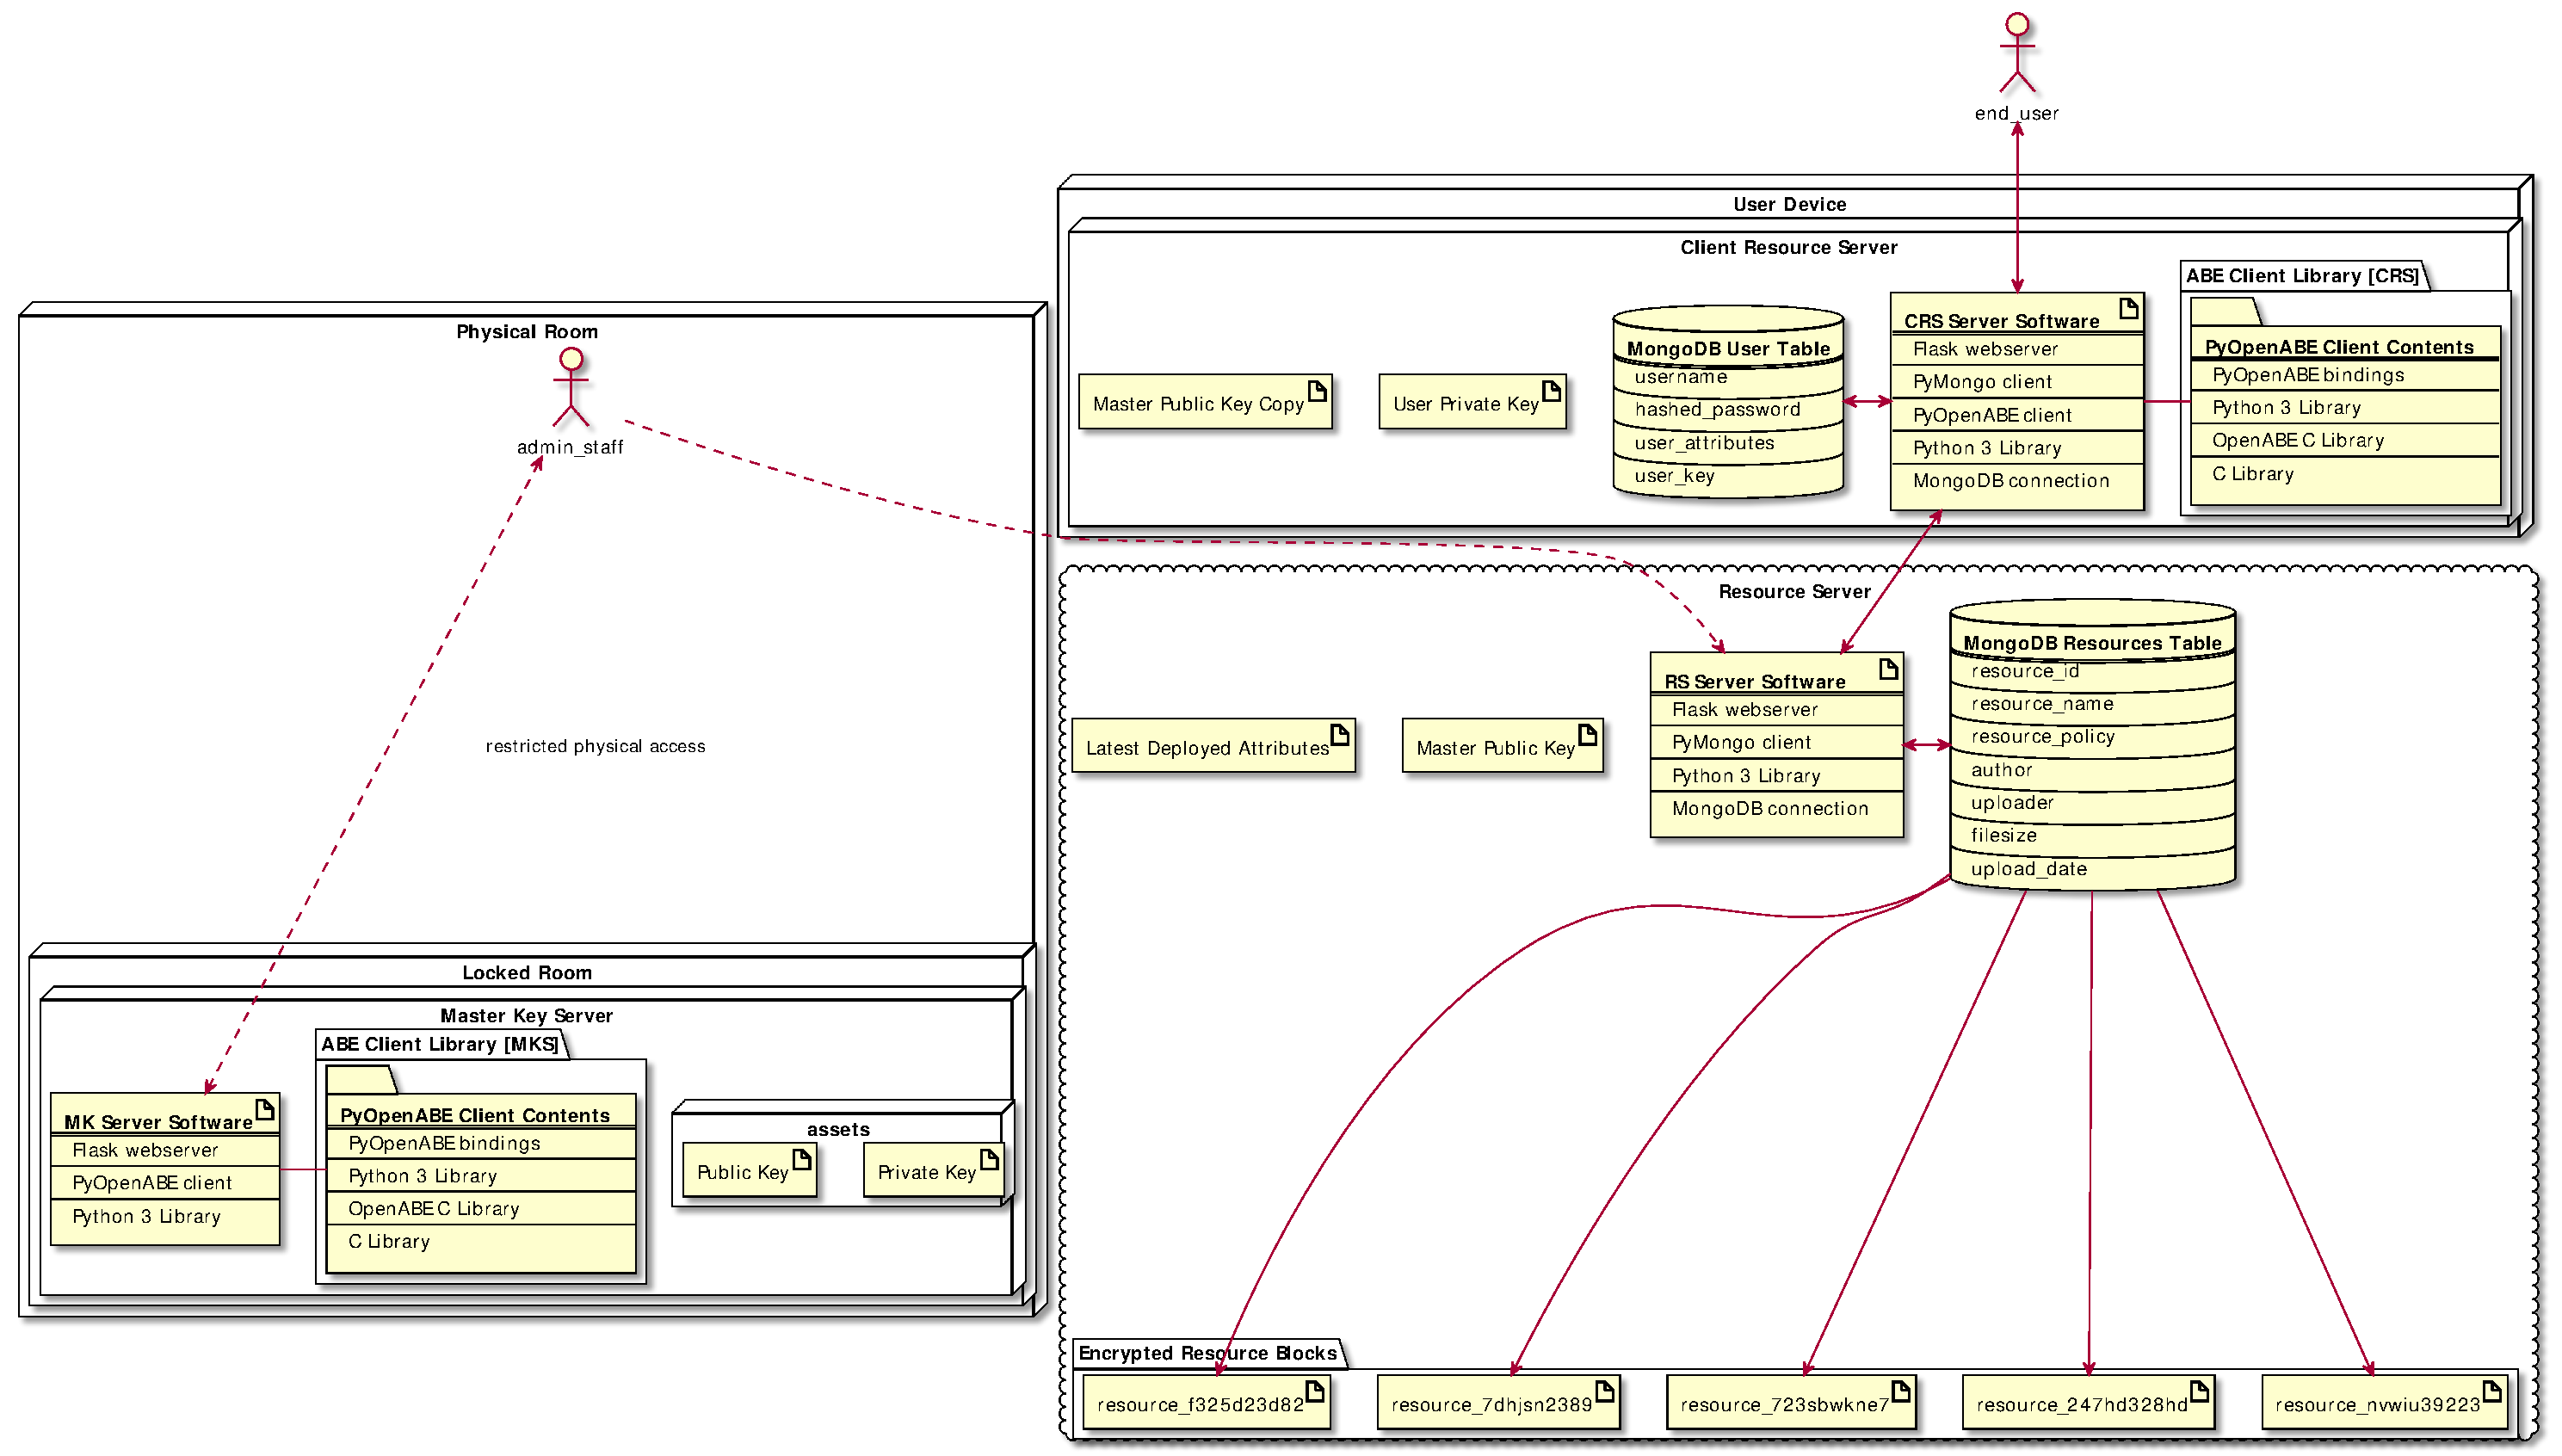
\includegraphics[width=\linewidth,keepaspectratio]{images/infrastructure/deployment.pdf}

    \caption{A deployment diagram of the \acrshort{dcs} \theResServer system. Both servers can be seen in context, with the master key server in its `offline' state and with physical access restricted to Admin staff. The public resource server is also shown receiving physical updates from the master key server (handled by Admin Staff) and communicating with client software running on a user's local device.}

    \label{fig:deployment_diagram}
\end{figure}

\subsection{Issuing User Keys}
\label{subsec:analysis_deployment_iuk}

From \cref{subsec:analysis_deployment_mks}, the master key server generates \& signs decryption keys for the \theResServer system, using the stored master \textbf{private} key. Further, as discussed in \cref{subsec:analysis_abe}, the decryption keys for the system are private user keys which contain embedded attributes that describe a user in terms that are defined by the organisation, which in this case is the \acrshort{dcs}.\\
For a user to start using the \theResServer system, they must enrol in the system by having a member of the \acrshort{dcs} Admin staff generate \& sign a new user key with their personal details from the master key server (see \cref{fig:enrolment_diagram} and appendix \ref{appendix:enrolment_diagram}). The key is created with attributes that should be retrieved from a department system such as MyCampus for students or the HR/Payroll system for staff. The master key server would be designed to \textit{validate} the attributes of a new user to ensure compatibility with encrypted resources and that all generated user keys are comparable.
\vskip 0.5em
However, the master key server would not be designed to \textit{verify} the attributes of a new user, since it is assumed that the Admin staff are responsible for verifying both the identity of a user and that the attributes about to be assigned to them are correct. The server would thus, implicitly trust that any inputs it receives have been verified and therefore, once validated would produce a new key; meaning both physical and login access to the server \textit{must only} be granted to trained members of staff.\\
In order for a user key to be provided to a new user, the Admin staff member must physically transfer the newly created key from the master server key to the student via some form of hardware storage such as a USB flash drive. Care would have to be taken to ensure that the master key server does not become infected from malicious storage devices that might be provided by a student.

\begin{figure}
    \centering
    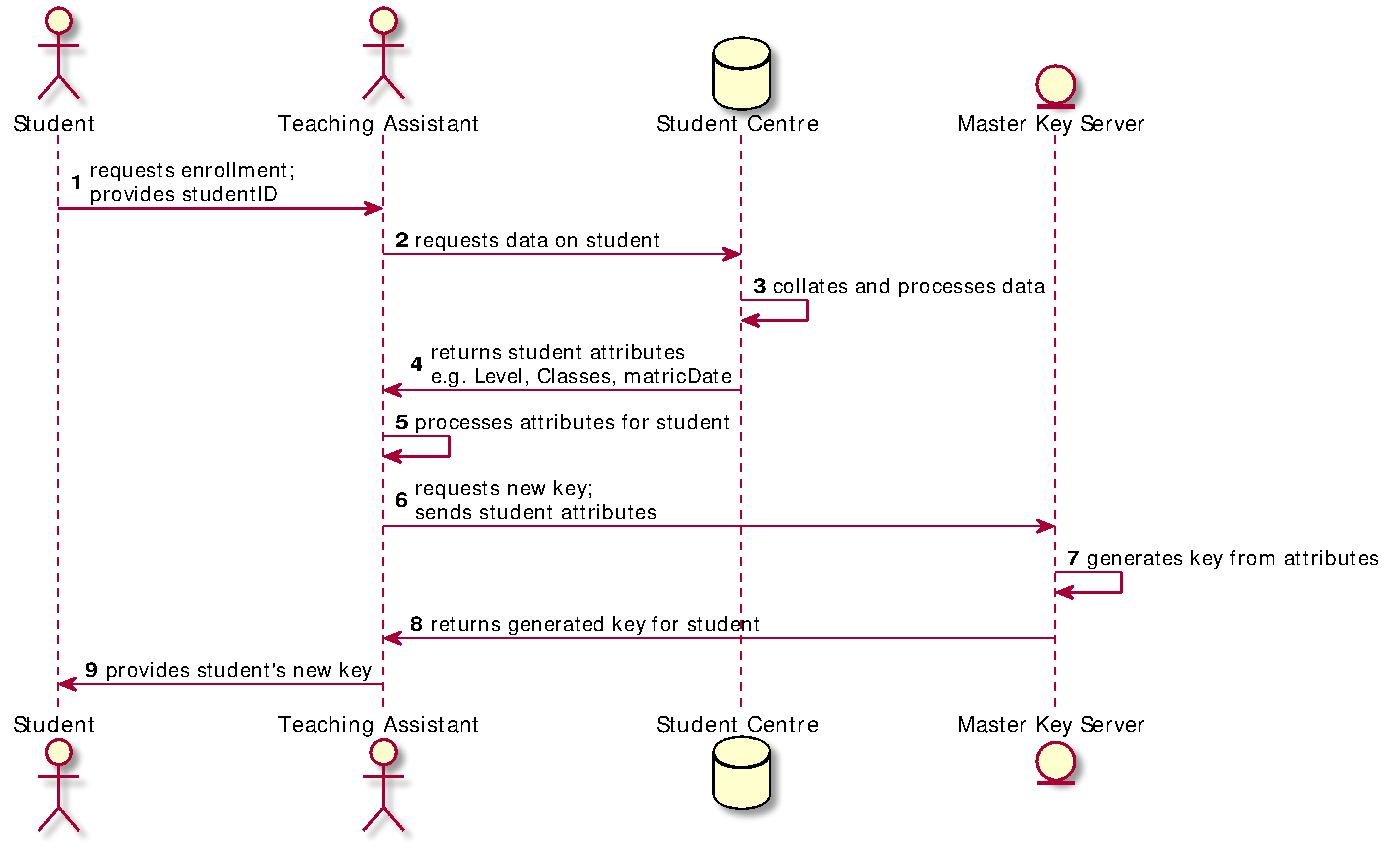
\includegraphics[width=\linewidth,keepaspectratio]{images/flow_of_info/enrollment_stu_sequence.pdf}

    \caption{A sequence diagram demonstrating the enrolment process for a student.
    The student can be seen requesting a user key \#1 (and providing their student ID) from the \acrshort{dcs} Teaching Assitant, whom verifies the student's identity and then retrieves their details \#2 from the Student Centre (or MyCampus) system. The Teaching Assistant then processes the returned attributes \#5 for the Master Key Server, and then requests a new key \#6 by providing the student's attributes. The Master Key Server can be seen processing \#7 and then returning the newly generated key \#8 to the Teaching Assistant, whom finally provides the key to the student.}

    \label{fig:enrolment_diagram}
\end{figure}


\section{Enrolment Requirements}
\label{sec:analysis_enrolment}

Following from \cref{subsec:analysis_deployment_mks} and \cref{subsec:analysis_deployment_iuk}, a Department of Computing Science user must be able to enrol in the \theResServer system by physically visiting the Teaching Office and proving their identity to the Admin staff. Staff and students could prove their identity with their respective campus ID cards, with passports providing further evidence should the Admin staff require it.\\
Any member of the \acrfull{dcs} would be eligible for enrolment in the system as long as they were able to adequately prove their membership to the Admin staff. This process would be deliberately designed to be partly physical for the added security in transferring the user's new key via a physical storage medium (instead of an electronic system such as email) as well as aiding the identity verification process with the user's physical presence.\\
New members of the \acrshort{dcs} must already physically attend an appointment to activate their campus cards for access to \acrshort{dcs} buildings \& laboratories, meaning that the \theResServer enrolment could reasonably be added to this process for limited impact on new users. Current users would have to visit the Teaching Office to complete enrolment into the system, however appointments could be timetabled and managed to ensure the smallest possible impact on \acrshort{dcs} members.


\section{Case Studies}
\label{sec:analysis_case_studies}

From the work completed in \cref{ch:background} and sections \ref{sec:analysis_security}, \ref{sec:analysis_deployment} \& \ref{sec:analysis_enrolment}, the project had determined the users of the resource server (see \cref{appendix:roles_users}) as well as the features the service would need to provide. With this information, several Case Studies were designed to demonstrate the extensibility of the system in real-world scenarios. Of the 6 Case Studies presented here, \cref{subsec:analysis_case_studies_3} and \cref{subsec:analysis_case_studies_4} are examined and discussed at the most in-depth level.

\subsection{\#0 \textemdash\ Past Exam Paper}
\label{subsec:analysis_case_studies_0}

Case Study \#0 considers a past exam paper uploaded as an encrypted resource by a member of the Administration staff for an arbitrary course. The staff member would like the past paper to be shared with all members of staff and students in the Department of Computing Science.
\vskip 0.5em
For this study the following details have been assumed:
\begin{itemize}
  \item
    the solutions were encrypted and then uploaded by the Admin staff member
  \item
    the staff member is Teresa Bonner with username `tbonner'
\end{itemize}
\vskip 0.5em
From the above information, we can identify attributes to be extracted for the policy, where we define \textbf{\textit{Subject} s} and \textbf{\textit{Environment} e} as:
\begin{itemize}
  \item[]
    \textbf{s} $\Rightarrow$ role, accountActiveUntil, username
  \item[]
    \textbf{e} $\Rightarrow$ currentDate
\end{itemize}

Applying the above attributes for the scenario provides the policy in \cref{fig:case_study_policy_0} which would have been embedded in the encrypted lecture slides by the staff member prior to upload. The encrypted past paper can then remain stored on the server but only accessible to staff members and students.

\begin{figure}[ht]
  \centering
\begin{align*}
  \text{Policy(\textbf{s},\textbf{e})}
  &
    \leftarrow
    \text{username(\textbf{s})} \equiv \text{`tbonner'}
  \\
  &
    \phantom{::}\vee
    \text{role(\textbf{s})} \equiv \text{`Staff'} \mid \text{`Student'}
  \\
  &
    \phantom{::}\wedge
    \text{accountActiveUntil(\textbf{s})} \geq \text{currentDate(\textbf{e})}
\end{align*}
  \caption{
    \label{fig:case_study_policy_0}
    Case Study \#0 policy dictating access to a past exam paper.
    Successful decryption would be possible for the author of the slides (with username `tbonner') \textbf{or} any member of staff \textbf{or} any student. In all cases an active account is also required.
  }
\end{figure}

\subsection{\#1 \textemdash\ Course Lecture Slides}
\label{subsec:analysis_case_studies_1}

Case Study \#1 considers a set of Lecture Slides uploaded as an encrypted resource by the Lecturer of an arbitrary course. The Lecturer would like the slides to be shared with other members of staff, to allow for suggestions and even collaboration, but only for Research \& Teaching staff. The Lecturer does not want the slides to be accessible to students until 24 hours before the scheduled lecture date, inline with university policy. For the sake of the scenario, the Java Programming 2 course was selected with Course Code 2001 in order to demonstrate the creation of a policy.
\vskip 0.5em
For this study the following details have been assumed:
\begin{itemize}
  \item
    the lecture slides have been uploaded in advance of the lecture date
  \item
    the lecture date is scheduled for 23/10/19
  \item
    the solutions were encrypted and then uploaded by the Lecturer
  \item
    the Lecturer for 2001 is Jeremy Springer with username `jspringer'
  \item
    Course 2001 is a Level 2 course
\end{itemize}
\vskip 0.5em
From the above information, we can identify attributes to be extracted for the policy, where we define \textbf{\textit{Subject} s} and \textbf{\textit{Environment} e} as:
\begin{itemize}
  \item[]
    \textbf{s} $\Rightarrow$ role, jobField, studentLevel, enrolledCourses, accountActiveUntil, username
  \item[]
    \textbf{e} $\Rightarrow$ currentDate
\end{itemize}

Applying the above attributes for the scenario provides the policy in \cref{fig:case_study_policy_1} which would have been embedded in the encrypted lecture slides by the Lecturer prior to upload. The encrypted slides can then remain stored on the server but only accessible to Research \& Teaching staff members until 24 hours before the lecture date of 23/10/19, when students on the course will also be granted access.

\begin{figure}[ht]
  \centering
\begin{align*}
  \text{Policy(\textbf{s},\textbf{e})}
  &
    \leftarrow
    \text{username(\textbf{s})} \equiv \text{`jspringer'}
  \\
  &
    \phantom{::}\vee
    \text{( role(\textbf{s})} \equiv \text{`Staff'}
  \\
  &
    \phantom{::::::::}\wedge
    \text{jobField(\textbf{s})} \equiv \text{`Research \& Teaching' )}
  \\
  &
    \phantom{::}\vee
    \text{( role(\textbf{s})} \equiv \text{`Student'}
  \\
  &
    \phantom{::::::::}\wedge
    \text{studentLevel(\textbf{s})} \equiv \text{2}
  \\
  &
    \phantom{::::::::}\wedge
    \text{enrolledCourses(\textbf{s})} \equiv \text{2001}
  \\
  &
    \phantom{::::::::}\wedge
    \text{currentDate(\textbf{e})} \geq \text{22 October 2019 )}
  \\
  &
    \phantom{::}\wedge
    \text{accountActiveUntil(\textbf{s})} \geq \text{currentDate(\textbf{e})}
\end{align*}
  \caption{
    \label{fig:case_study_policy_1}
    Case Study \#1 policy dictating access to a set of course 2001 lecture slides.
    Successful decryption would be possible for the author of the slides (with username `jspringer') \textbf{or} a member of staff in the Research \& Teaching field \textbf{or} a Level 2 student enrolled in the 2001 course if the lecture slides' release date has passed. In all cases an active account is also required.
  }
\end{figure}

\subsection{\#2 \textemdash\ Course Lab Solutions}
\label{subsec:analysis_case_studies_2}

Case Study \#2 considers a lab solution uploaded as an encrypted resource by the Lecturer of an arbitrary course. The Lecturer would like to upload the solutions in advance of the lab date, allowing for other members of staff to verify the solutions, but only for Research \& Teaching staff. The Lecturer does not want the solutions to be accessible to students until 3 days after the scheduled lab date, allowing the Lecturer to talk through the solutions in a lecture before release. The Lecturer would like the solutions to be available to tutors \& demonstrators that will be assisting in the lab, so that they can properly offer help to students.\\
For the sake of the scenario, the 1P Programming course was selected with Course Code 1001 as it offers the added complexity of tutors \& demonstrators, but it should be remembered that any course with labs could have been chosen.
\vskip 0.5em
For this study the following details have been assumed:
\begin{itemize}
  \item
    the lab solutions have been uploaded in advance of the actual lab date
  \item
    the lab date is scheduled for 04/12/19
  \item
    the solutions were encrypted and then uploaded by the Lecturer
  \item
    the Lecturer for 1001 is John Williamson with username `jwilliamson'
  \item
    Course 1001 is a Level 1 course
  \item
    Course 1001 has a sister course, 1017
  \item
    the 1P course labs are assisted by tutors \& demonstrators from Level 4+
\end{itemize}
\vskip 0.5em
From the above information, we can identify attributes to be extracted for the policy, where we define \textbf{\textit{Subject} s} and \textbf{\textit{Environment} e} as:
\begin{itemize}
  \item[]
    \textbf{s} $\Rightarrow$ role, jobField, studentLevel, enrolledCourses, accountActiveUntil, startDate, endDate, username, studentRole, demonstratorCourses
  \item[]
    \textbf{e} $\Rightarrow$ currentDate
\end{itemize}

Applying the above attributes for the scenario provides the policy in \cref{fig:case_study_policy_2} which would have been embedded in the encrypted lab solution by the Lecturer prior to upload. The encrypted lab solution can then remain stored on the server but only accessible to Research \& Teaching staff members and valid tutors \& demonstrators until 3 days after the lab date of 04/12/19, when students on the course will also be granted access.

\begin{figure}[ht]
  \centering
\begin{align*}
  \text{Policy(\textbf{s},\textbf{e})}
  &
    \leftarrow
    \text{username(\textbf{s})} \equiv \text{`jwilliamson'}
  \\
  &
    \phantom{::}\vee
    \text{( role(\textbf{s})} \equiv \text{`Staff'}
  \\
  &
    \phantom{::::::::}\wedge
    \text{jobField(\textbf{s})} \equiv \text{`Research \& Teaching' )}
  \\
  &
    \phantom{::}\vee
    \text{( role(\textbf{s})} \equiv \text{`Student'}
  \\
  &
    \phantom{::::::::}\wedge
    \text{studentLevel(\textbf{s})} \equiv \text{1}
  \\
  &
    \phantom{::::::::}\wedge
    \text{enrolledCourses(\textbf{s})} \equiv \text{[1001, 1017]}
  \\
  &
    \phantom{::::::::}\wedge
    \text{currentDate(\textbf{e})} \geq \text{7 December 2019 )}
  \\
  &
    \phantom{::}\vee
    \text{( role(\textbf{s})} \equiv \text{`Student'}
  \\
  &
    \phantom{::::::::}\wedge
    \text{studentLevel(\textbf{s})} \geq \text{4}
  \\
  &
    \phantom{::::::::}\wedge
    \text{studentRole(\textbf{s})} \equiv \text{`Demonstrator UG'} \mid \text{`Demonstrator PG'} \mid \text{`Tutor'}
  \\
  &
    \phantom{::::::::}\wedge
    \text{demonstratorCourses(\textbf{s})} \equiv \text{[1001, 1017]}
  \\
  &
    \phantom{::::::::}\wedge
    \text{startDate(\textbf{e})} \leq \text{currentDate(\textbf{e})}
  \\
  &
    \phantom{::::::::}\wedge
    \text{endDate(\textbf{e})} \geq \text{currentDate(\textbf{e}) )}
  \\
  &
    \phantom{::}\wedge
    \text{accountActiveUntil(\textbf{s})} \geq \text{currentDate(\textbf{e})}
\end{align*}
  \caption{
    \label{fig:case_study_policy_2}
    Case Study \#2 policy dictating access to a set of course `1001' lab solutions.
    Successful decryption would be possible for the author of the solutions (with username `jwilliamson') \textbf{or} a member of staff in the `Research \& Teaching' field \textbf{or} a Level 2 student enrolled in the `1001' \& `1017' courses if the lab date has passed \textbf{or} a Level 4+ student employed as a demonstrator or tutor that has been assigned to the `1001' \& `1017' course and it is within their dates of employment. In all cases an active account is also required.
  }
\end{figure}

\subsection{\#3 \textemdash\ In-progress Exam Script}
\label{subsec:analysis_case_studies_3}

Case Study \#3 considers an in-progress exam script uploaded as an encrypted resource by the Lecturer of an arbitrary course. The exam script is still a draft and is currently being worked on by one or more members of staff in preparation for the exam period. The Lecturer would like to upload the script in advance of the exam date, allowing for other members of staff to verify the script and offer feedback, but only for Research \& Teaching staff.\\
The script is considered confidential and should only accessible to staff within the Lecturer's Research Group (e.g. FATA, GLASS, IDA) and more specifically their Theme\slash Topic group (e.g. FDTST, MOG, HUSH), unless the Lecturer has specifically granted an individual access. The exam script must also be accessible to Admin staff so that it can be passed to the Exam board for final review. The exam has a scheduled date and a following marking period in which markers will also need access.\\
For the sake of the scenario, the Programming Languages course was selected with Course Code 4016 in order to demonstrate the creation of a policy.
\vskip 0.5em
For this study the following details have been assumed:
\begin{itemize}
  \item
    the exam script is a work in progress resource
  \item
    the exam script has been uploaded in advance of the exam date
  \item
    the solutions were encrypted and then uploaded by the Lecturer
  \item
    the Lecturer's Research Group is FATA
  \item
    the Lecturer's Research Theme\slash Topic is Programming Languages
  \item
    the exam date is 12/05/20
  \item
    the marking deadline is 10/06/20
  \item
    the Lecturer for 4016 is Ornela Dardha with username `odardha'
  \item
    collaborators include Simon Gay (`sgay'), John O'Donnell (`jodonnell')
\end{itemize}
\vskip 0.5em
From the above information, we can identify attributes to be extracted for the policy, where we define \textbf{\textit{Subject} s} and \textbf{\textit{Environment} e} as:
\begin{itemize}
  \item[]
    \textbf{s} $\Rightarrow$ role, jobField, jobRole, researchGroup, researchTheme, accountActiveUntil, staffRole, markerFrom, markerTo, markerCourses, username
  \item[]
    \textbf{e} $\Rightarrow$ currentDate
\end{itemize}

Applying the above attributes for the scenario provides the policy in \cref{fig:case_study_policy_3} which would have been embedded in the encrypted exam script by the Lecturer prior to upload. The encrypted exam script can then remain stored on the server but would only be the Lecturer themselves, as well as the specified collaborators.\\
Further access would be granted to staff members in the Professional, Administrative \& Support field that specifically have the Administration role, as well as Research \& Teaching staff members that belong to the FATA research group and the Programming Languages research theme. Lastly, access would be granted to markers that have been assigned to the 4016 course and will be actively marking during the marking period (12/05/20-10/06/20).

\begin{figure}[ht]
  \centering
\begin{align*}
  \text{Policy(\textbf{s},\textbf{e})}
  &
    \leftarrow
    \text{username(\textbf{s})} \equiv \text{`odardha'} \mid \text{`sgay'} \mid \text{`jodonnell'}
  \\
  &
    \phantom{::}\vee
    \text{( role(\textbf{s})} \equiv \text{`Staff'}
  \\
  &
    \phantom{::::::::}\wedge
    \text{jobField(\textbf{s})} \equiv \text{`Professional, Administrative \& Support'}
  \\
  &
    \phantom{::::::::}\wedge
    \text{jobRole(\textbf{s})} \equiv \text{`Administration' )}
  \\
  &
    \phantom{::}\vee
    \text{( role(\textbf{s})} \equiv \text{`Staff'}
  \\
  &
    \phantom{::::::::}\wedge
    \text{jobField(\textbf{s})} \equiv \text{`Research \& Teaching'}
  \\
  &
    \phantom{::::::::}\wedge
    \text{researchGroup(\textbf{s})} \equiv \text{`FATA'}
  \\
  &
    \phantom{::::::::}\wedge
    \text{researchTheme(\textbf{s})} \equiv \text{`Programming Languages' )}
  \\
  &
    \phantom{::}\vee
    \text{( role(\textbf{s})} \equiv \text{`Staff'}
  \\
  &
    \phantom{::::::::}\wedge
    \text{staffRole(\textbf{s})} \equiv \text{`Marker'}
  \\
  &
    \phantom{::::::::}\wedge
    \text{markerFrom(\textbf{s})} \geq \text{12 May 2020}
  \\
  &
    \phantom{::::::::}\wedge
    \text{markerTo(\textbf{s})} \leq \text{10 June 2020}
  \\
  &
    \phantom{::::::::}\wedge
    \text{markerCourses(\textbf{s})} \equiv \text{4016}
  \\
  &
    \phantom{::}\wedge
    \text{accountActiveUntil(\textbf{s})} \geq \text{currentDate(\textbf{e})}
\end{align*}
  \caption{
    \label{fig:case_study_policy_3}
    Case Study \#3 policy dictating access to a work-in-progress exam script for course `4016'.
    Successful decryption would be possible for the author of the solutions (with username `odardha') as well as the named collaborators (with usernames `sgay' \& `jodonnell') \textbf{or} for a member of staff in the `Professional, Administrative \& Support' field with the `Administration' role \textbf{or} for a member of staff in the `Research \& Teaching' field that is also in the `FATA' research group and the `Programming Languages' research theme \textbf{or} for a member of staff with the `Marker' role that is assigned to marking duties within the marking period and has been assigned to the `4016' course. In all cases an active account is also required.
  }
\end{figure}

\subsection{\#4 \textemdash\ Level 4 Honours Individual Project}
\label{subsec:analysis_case_studies_4}

Case Study \#4 considers a completed individual project from a Level 4 student, particularly the dissertation resource although the project source code could also be treated identically if submitted as a compressed .tar.gz or .zip file.\\
In this case, the student has encrypted and uploaded their dissertation to the resource server with access to be granted for their supervisor, the assigned reader and additionally, the Project Coordinator.
\vskip 0.5em
For this study the following details have been assumed:
\begin{itemize}
  \item
    the student has the ID and username `2123456z'
  \item
    their supervisor is Quintin Cutts with username `qcutts'
  \item
    their assigned reader is Paul Siebert with username `psiebert'
  \item
    the Project Coordinator is John Williamson with username `jwilliamson'
\end{itemize}
\vskip 0.5em
From the above information, we can identify attributes to be extracted for the policy, where we define \textbf{\textit{Subject} s} and \textbf{\textit{Environment} e} as:
\begin{itemize}
  \item[]
    \textbf{s} $\Rightarrow$ role, accountActiveUntil, username
  \item[]
    \textbf{e} $\Rightarrow$ currentDate
\end{itemize}

Applying the above attributes for the scenario provides the policy in \cref{fig:case_study_policy_4} which would have been embedded in the encrypted dissertation by the student prior to upload. The encrypted dissertation can then remain stored on the server but only accessible to the student and required staff members.

\begin{figure}[ht]
  \centering
\begin{align*}
  \text{Policy(\textbf{s},\textbf{e})}
  &
    \leftarrow
    \text{( role(\textbf{s})} \equiv \text{`Student'}
  \\
  &
    \phantom{::::::}\wedge
    \text{username(\textbf{s})} \equiv \text{`2123456z' )}
  \\
  &
    \phantom{::}\vee
    \text{( role(\textbf{s})} \equiv \text{`Staff'}
  \\
  &
    \phantom{::::::}\wedge
    \text{username(\textbf{s})} \equiv \text{`qcutts'} \mid \text{`psiebert'} \mid \text{`jwilliamson' )}
  \\
  &
    \phantom{::}\wedge
    \text{accountActiveUntil(\textbf{s})} \geq \text{currentDate(\textbf{e})}
\end{align*}
  \caption{
    \label{fig:case_study_policy_4}
    Case Study \#4 policy dictating access to a completed dissertation.
    Successful decryption would be possible for the author of the dissertation (with username `2123456z') \textbf{or} for the 3 identified staff members (with usernames `qcutts', `psiebert', `jwilliamson'). In all cases an active account is also required.
  }
\end{figure}


\subsection{\#5 \textemdash\ Class Representative Meeting Minutes}
\label{subsec:analysis_case_studies_5}

Case Study \#5 considers the secure storage of the minutes from a Class Representative meeting, which would have been uploaded as an encrypted resource by a member of Admin staff after recording. The minutes should be accessible to all Research \& Teaching staff as well as the rest of the Administration team. Further, all active class reps should also have access to the minutes, as it is assumed that they will have attended the meeting. Lastly, the Head of the DCS (Head of School) should also have access to the minutes to see what was discussed \& decided.\\
In this case, the member of staff has encrypted and uploaded the minutes to the resource server with access granted as above.
\vskip 0.5em
For this study the following details have been assumed:
\begin{itemize}
  \item
    the member of staff is Tania Galabova with username `tgalabova'
  \item
    the meeting occurred on 12/09/19
\end{itemize}
\vskip 0.5em
From the above information, we can identify attributes to be extracted for the policy, where we define \textbf{\textit{Subject} s} and \textbf{\textit{Environment} e} as:
\begin{itemize}
  \item[]
    \textbf{s} $\Rightarrow$ role, accountActiveUntil, username
  \item[]
    \textbf{e} $\Rightarrow$ currentDate
\end{itemize}

Applying the above attributes for the scenario provides the policy in \cref{fig:case_study_policy_5} which would have been embedded in the encrypted minutes by the member of staff prior to upload. The encrypted minutes can then remain stored on the server but will only be accessible to Research \& Teaching staff members, Administration staff members and the current Head of School. Further access would also be granted to students currently serving as Class Representatives.

\begin{figure}[ht]
  \centering
\begin{align*}
  \text{Policy(\textbf{s},\textbf{e})}
  &
    \leftarrow
    \text{username(\textbf{s})} \equiv \text{`tgalabova'}
  \\
  &
    \phantom{::}\vee
    \text{( role(\textbf{s})} \equiv \text{`Staff'}
  \\
  &
    \phantom{::::::::}\wedge
    \text{jobField(\textbf{s})} \equiv \text{`Research \& Teaching' )}
  \\
  &
    \phantom{::}\vee
    \text{( role(\textbf{s})} \equiv \text{`Staff'}
  \\
  &
    \phantom{::::::::}\wedge
    \text{jobField(\textbf{s})} \equiv \text{`Professional, Administrative \& Support'}
  \\
  &
    \phantom{::::::::}\wedge
    \text{jobRole(\textbf{s})} \equiv \text{`Administration' )}
  \\
  &
    \phantom{::}\vee
    \text{( role(\textbf{s})} \equiv \text{`Staff'}
  \\
  &
    \phantom{::::::::}\wedge
    \text{staffRole(\textbf{s})} \equiv \text{`Head of School'}
  \\
  &
    \phantom{::::::::}\wedge
    \text{headSchoolFrom(\textbf{s})} \geq \text{17 Sep 2019}
  \\
  &
    \phantom{::::::::}\wedge
    \text{headSchoolTo(\textbf{s})} \leq \text{16 Sep 2020 )}
  \\
  &
    \phantom{::}\vee
    \text{( role(\textbf{s})} \equiv \text{`Student'}
  \\
  &
    \phantom{::::::::}\wedge
    \text{studentRole(\textbf{s})} \equiv \text{`Class Representative'}
  \\
  &
    \phantom{::::::::}\wedge
    \text{classRepFrom(\textbf{s})} \geq \text{17 Sep 2019}
  \\
  &
    \phantom{::::::::}\wedge
    \text{classRepTo(\textbf{s})} \leq \text{16 Sep 2020 )}
  \\
  &
    \phantom{::}\wedge
    \text{accountActiveUntil(\textbf{s})} \geq \text{currentDate(\textbf{e})}
\end{align*}
  \caption{
    \label{fig:case_study_policy_5}
    Case Study \#5 policy dictating access to a Class Rep meeting minutes.
    Successful decryption would be possible for the author of the minutes (with username `tgalabova') \textbf{or} for any `Research \& Teaching' staff members \textbf{or} for any `Administration' staff members \textbf{or} for the `Head of School', if their serving term matches the academic year of the minutes \textbf{or} for any students serving as a `Class Representative' in the academic year of the minutes. In all cases an active account is also required.
  }
\end{figure}


%==================================================================================================================================
\chapter{Design}
\label{ch:design}

\section{Requirements}
\label{sec:design_reqs}

\subsection{Deployment}

The resource server product was designed around the specific deployment scenario of the Department of Computing Science (DCS) and as such, aims to meet the requirements of users belonging to the DCS. Identified by an analysis of the DCS structure, considering students, teaching staff, technical staff \& admin staff and identifying both key roles and individuals within the organisation (see \ref{appendix:roles_users}).\\
Subsequently, the resource server focuses on the secure distribution of resources between members of a department with particular emphasis on the sharing of course resources between members of staff and the students taking their course(s).
\vskip 0.5em
This scenario also lends itself well to proving the the extensibility of the product as students have varying and changing attributes that are assigned in their private user keys - the dynamic nature of which allows the product to maintain a high level of portability.\\
This granularity in attributes, and thus policies, also provides long-term support for the product by allowing it to adapt to future changes in user structure and policy requirements.\\
Further, allowing the system to be deployed to completely new environments as the attributes can be unique to an industry and do not require definition prior to deployment.
\vskip 0.5em
The product was thus determined to require one central master key server, tasked with maintaining the master private key, provisioning the corresponding master public key and using said private key to sign new user keys.\\
A second server would handle the distribution of the master public key, storage of the encrypted resources and serving \& receiving encrypted resources.\\
Further, it was determined that for the DCS deployment, the master key server would serve as an offline or 'cold' server with no internet connection; as this provides a strong level of base security against external threats. Such offline status is possible because the master key server is not required to distribute data automatically, but rather the master public key can be manually uploaded to the resource server.

\subsection{ABE System}

As described earlier, an ABE system requires a defined policy language in order to build policies for resources to be encrypted with. This policy language describes the syntax and types of policies and is tailored to the deployment above by allowing for attributes that are required for students and staff of the DCS.\\
The ABE system required an ABE library for implementation, however since creating such a library was beyond the scope of the project, the \href{https://github.com/zeutro/openabe}{OpenABE library} from Zeutro LLC was selected instead. OpenABE was selected based upon the open source philosophy it adopts and the demonstration of its deployment as an electronic medical record system \cite{Akinyele2011}. A system that aligns well with that of a secure, departmental resource server but with even greater requirements for security.

\subsection{Resources}

Since uploaded resources have to be securely encrypted with ABE before transmission, the resource server is unaware of the contents of all resources and is in the disadvantaged position of being unable to help users identify which resources are which.\\
As such, the server must utilise a different method for resource identification and instead relies on an internal database to store metadata of resources as provided when a user performs an upload. This metadata includes filename, extension, file size and author, but most importantly keeps a record of the resource's policy in order to determine if a user should even be able to download the resource.\\
Importantly, any user \textit{could} download \textit{any} encrypted resource without risk of unauthorised decryption, however the user experience would be


\section{Formal Language Definition}
\label{sec:formal_lang}

We offer the following formal language definition for the resource server's Attribute-Based Encryption policy language, \thePolicyLang. The language was designed around the Case Studies described in \cref{sec:analysis_case_studies} and follows an extensible design principle that aims to provide a complete policy solution for the Department of Computing Science.\\
\thePolicyLang directly provides the tools for policies to be constructed for the \cref{sec:analysis_case_studies} Case Studies, which can then be interpreted to the policy format that the PyOpenABE python bindings (described in \cref{sec:bkgr_openabe}) require.
\vskip 0.5em
\thePolicyLang offers boolean comparisons for integer, string \& date attributes with further support for lists of multiple values. Additional comparison operations are provided for integer and date comparisons with `greater than', `less than' and `equivalent to' all supported, whereas booleans, strings and lists support `equivalent to' operations only.\\
This allows for integer comparisons such as ``\textit{studentLevel(\textbf{s}) $\geq$ 4}'' (as found in Case Study \#2, \cref{fig:case_study_policy_2}) and date comparisons such as ``\textit{classRepFrom(\textbf{s}) $\geq$ 17 Sep 2019}'' (as found in Case Study \#5, \cref{fig:case_study_policy_5}). String equivalence operations allow for comparisons such as ``\textit{jobField(\textbf{s}) $\equiv$ `Research \& Teaching'}'' (as found in Case Study \#1, \cref{fig:case_study_policy_1}).\\
List equivalence operations are also supported, allowing for comparisons such as ``\textit{enrolledCourses(\textbf{s}) $\equiv$ [1001, 1017]}'' (as found in Case Study \#2 \cref{fig:case_study_policy_2}) where the policy requires both that `\textit{enrolledCourses(\textbf{s})}' resolves to a list and that that list contains the elements in `\textit{[1001, 1017]}'.

\section{Abstract Syntax, Types, \& Contexts}\label{sec:defs}

\begin{figure}[ht]
  \centering
\begin{align*}
  \ty{n}{\mathbb{Z}}
  &
    \Coloneqq
    \text{Integers}
  & \text{Values}
  \\
  \ty{b}{\mathbb{B}}
  & \Coloneqq
    \mathsf{False}\alt\mathsf{True}
  \\
  \ty{d}{\mathbb{D}}
  & \Coloneqq
    \text{Dates}
  \\
  \ty{s}{\mathbb{S}}
  & \Coloneqq
    \text{Strings}
  \\
  v
  &
    \Coloneqq
    n
    \alt
    b
    \alt
    d
    \alt
    s
  \\
  \ty{l}{\mathbb{L}_T}
  & \Coloneqq
    \emptyset_T\alt{}v\Cons_T{}l
  \\
  e
  &
    \Coloneqq
    v
    \alt
    l
  & \text{Expressions}
  \\
  &
    \firstAlt
    \exprEQ{e}{e}
    \alt
    \exprGT{e}{e}
    \alt
    \exprLT{e}{e}
  \\
  & \firstAlt
    \exprGTE{e}{e}
    \alt
    \exprLTE{e}{e}
  &
  \\
  & \firstAlt
    \exprOr{e}{e}
    \alt
    \exprAnd{e}{e}
  &
  \\
  &
    \firstAlt
    \left( \lambda \mu \bullet e \right)
    \alt
    e \; \$ \; e
  &
    \text{Statements}
  \\
  T
  &
    \Coloneqq
    \mathbb{Z}
    \alt
    \mathbb{B}
    \alt
    \mathbb{D}
    \alt
    \mathbb{S}
    \alt
    \mathbb{L}
    \alt
    {T \rightarrow{} T}
  &
    \text{Types}
  \\
  \Gamma
  &
    \Coloneqq
    \envAdd{(\ty{x}{T})}
    \alt
    \emptyset
    &
      \text{Context}
\end{align*}
  \caption{\label{fig:syntax}The policy language's abstract syntax, types, and context.}
\end{figure}

\Cref{fig:syntax} presents the syntactical structure, and types for our language.
Our language contains Integers, Boolean, Date, String and List values, we leave abstract how integers and dates are written.

Integers \& Dates can be compared using standard comparison operations of: \texttt{greater-than}, \texttt{less-than} and \texttt{equals-to}, as well as \texttt{greater-than-or-equal-to} and \texttt{less-than-or-equal-to}.
Boolean operators provide logical conjunction and disjunction.

A context ($\Gamma$) keeps track of well-typed expressions, and our context can be expanded.


\subsection{Typing Rules}
\label{subsec:typing-rules}

\begin{figure}[ht]
  \centering
\begin{mathpar}
  \infer*[left=Intro-Int]
  {
    \\
  }
  {
    \ty{i}{\TyInt}
  }
  \and
  \infer*[left=Intro-Bool]
  {
    \\
  }
  {
    \ty{b}{\mathbb{B}}
  }
  \and
  \infer*[left=Intro-Date]
  {
    \\
  }
  {
    \ty{d}{\mathbb{D}}
  }
  \and
  \infer*[left=Intro-String]
  {
    \\
  }
  {
    \ty{s}{\mathbb{S}}
  }
  \and
  \infer*[left=Intro-Empty]
  {
    \env{\ty{a}{T}}\\
    \left[ T \in T_l \right]
  }
  {
    \env{\ty{\emptyset_a}{\mathbb{L}_a}}
  }
  \and
  \infer*[left=Intro-Cons]
  {
    \env{\ty{v}{a}}\\
    \env{\ty{l}{\mathbb{L}_a}}\\
    \env{\ty{a}{T}}\\
    \left[ T \in T_l \right]
  }
  {
    \env{\ty{v\Cons_t{}l}{\mathbb{L}_a}}
  }
  \and
  \infer*[left=OR]
  {
    \env{\ty{a}{\mathbb{B}}}\\
    \env{\ty{b}{\mathbb{B}}}
  }
  {
    \env{\ty{\exprOr{a}{b}}{\mathbb{B}}}
  }
  \and
  \infer*[left=AND]
  {
    \env{\ty{a}{\mathbb{B}}}\\
    \env{\ty{b}{\mathbb{B}}}
  }
  {
    \env{\ty{\exprAnd{a}{b}}{\mathbb{B}}}
  }
  \and
  \infer*[left=GT]
  {
    \env{\ty{a}{T}}\\
    \env{\ty{b}{T}}\\
    \left[ T \in \{ \mathbb{Z}, \mathbb{D} \} \right]
  }
  {
    \env{\ty{\exprGT{a}{b}}{\mathbb{B}}}
  }
  \and
  \infer*[left=LT]
  {
    \env{\ty{a}{T}}\\
    \env{\ty{b}{T}}\\
    \left[ T \in \{ \mathbb{Z}, \mathbb{D} \} \right]
  }
  {
    \env{\ty{\exprLT{a}{b}}{\mathbb{B}}}
  }
  \and
  \infer*[left=EQ]
  {
    \env{\ty{a}{T}}\\
    \env{\ty{b}{T}}\\
    \left[ T \in \{ \mathbb{Z}, \mathbb{B}, \mathbb{D}, \mathbb{S}, \mathbb{L}_t \} \right]
  }
  {
    \env{\ty{\exprEQ{a}{b}}{\mathbb{B}}}
  }
  \and
  \infer*[left=GTE]
  {
    \env{\ty{a}{T}}\\
    \env{\ty{b}{T}}\\
    \left[ T \in \{ \mathbb{Z}, \mathbb{D} \} \right]
  }
  {
    \env{\ty{\exprGTE{a}{b}}{\mathbb{B}}}
  }
  \and
  \infer*[left=LTE]
  {
    \env{\ty{a}{T}}\\
    \env{\ty{b}{T}}\\
    \left[ T \in \{ \mathbb{Z}, \mathbb{D} \} \right]
  }
  {
    \env{\ty{\exprLTE{a}{b}}{\mathbb{B}}}
  }
\end{mathpar}
  \caption{\label{fig:rules}The formal definition of the Typing Rules for \thePolicyLang}
\end{figure}

\Cref{fig:rules} presents the \thePolicyLang typing rules.
These rules dictate what it means for an expression/statement to be well-formed within \thePolicyLang and for any expression/statement in \thePolicyLang, we use the typing rules to construct a derivation that provides proof that the expression/statement is well-typed, that is we can apply each rule and form a derivation tree. If we cannot construct this tree then the expression is ill-typed and syntactically not valid.

The Typing Rules define 5 base cases for the 5 value types \thePolicyLang supports (as defined in \cref{fig:syntax}), meaning instances of the 5 types derive directly to their type. Next, the boolean logical operators OR \& AND are defined as requiring two Boolean parameters that also derive to a Boolean type return. The standard comparison operators \textbf{$>$}, \textbf{$<$}, \textbf{$>=$} \& \textbf{$<=$} all take two parameters of a matching type, where the type may be Integer or Date, and derives to a Boolean response. Lastly, the \textbf{$==$} comparison similarly takes two parameters of a matching type, but where the type may be Integer, Boolean, Date, String or List, and also derives to a Boolean return.


\subsection{Substitution}
\label{subsec:substitution}

\begin{figure}[ht]
  \centering
\begin{align*}
  \subst{\mu}{e}{x}
  &
    \Coloneqq
    \begin{cases}
      e&x\equiv\mu\\
      x&x\not\equiv\mu\\
    \end{cases}
  \\
  \subst{\exprOr{a}{b}}{e}{x}&\Coloneqq\exprOr{\subst{a}{e}{x}}{\subst{b}{e}{x}}\\
  \subst{\exprAnd{a}{b}}{e}{x}&\Coloneqq\exprAnd{\subst{a}{e}{x}}{\subst{b}{e}{x}}\\
  \subst{\exprGT{a}{b}}{e}{x}&\Coloneqq\exprGT{\subst{a}{e}{x}}{\subst{b}{e}{x}}\\
  \subst{\exprLT{a}{b}}{e}{x}&\Coloneqq\exprLT{\subst{a}{e}{x}}{\subst{b}{e}{x}}\\
  \subst{\exprEQ{a}{b}}{e}{x}&\Coloneqq\exprEQ{\subst{a}{e}{x}}{\subst{b}{e}{x}}\\
  \subst{\exprGTE{a}{b}}{e}{x}&\Coloneqq\exprGTE{\subst{a}{e}{x}}{\subst{b}{e}{x}}\\
  \subst{\exprLTE{a}{b}}{e}{x}&\Coloneqq\exprLTE{\subst{a}{e}{x}}{\subst{b}{e}{x}}
\end{align*}
  \caption{\label{fig:subst}The formal definition of the Substitution Rules for \thePolicyLang}
\end{figure}

\Cref{fig:subst} presents a standard set of substitution rules for \thePolicyLang.
These rules describe how we can iterate over our expressions/statements in \thePolicyLang and through recursive calls, swap variables for values.\\
Starting with expressions and variables, we describe when $\mu$ is an expression or variable. Next we describe the resolving of the \textbf{or} \& \textbf{and} logical operators' parameters to expressions and variables, followed by similar descriptions for the standard comparisons \textbf{greaterThan}, \textbf{lessThan}, \textbf{equal}, \textbf{greaterThanEqual} \& \textbf{lessThanEqual}.\\
Through the recursive calls, we eventually reach a state where we have visited all expressions \& statements and we can swap in values in place of all variables by working backwards through the recursive calls.


\subsection{Big Step Semantics}
\label{subsec:semantics}

\begin{figure}[ht]
  \centering
\begin{mathpar}
  \infer*[left=$\mathbb{Z}$]
  {
    \\
  }
  {
    i\Downarrow{}\primed{i}
  }
  \and
  \infer*[left=$\mathbb{B}$]
  {
    \\
  }
  {
    b\Downarrow{}\primed{b}
  }
  \and
  \infer*[left=$\mathbb{D}$]
  {
    \\
  }
  {
    d\Downarrow{}\primed{d}
  }
  \and
  \infer*[left=$\mathbb{S}$]
  {
    \\
  }
  {
    s\Downarrow{}\primed{s}
  }
  \and
  \infer*[left=$\mathbb{L}$]
  {
    \\
  }
  {
    l\Downarrow{}\primed{l}
  }
  \and
  \infer*[left=OR]
  {
    a\Downarrow{}\primed{a}\\
    b\Downarrow{}\primed{b}
  }
  {
    \exprOr{a}{b}\Downarrow\primed{a}\vee\primed{b}
  }
  \and
  \infer*[left=AND]
  {
    a\Downarrow{}\primed{a}\\
    b\Downarrow{}\primed{b}
  }
  {
    \exprAnd{a}{b}\Downarrow\primed{a}\wedge\primed{b}
  }
  \and
  \infer*[left=GT]
  {
    a\Downarrow{}\primed{a}\\
    b\Downarrow{}\primed{b}
  }
  {
    \exprGT{a}{b}\Downarrow\primed{a}>\primed{b}
  }
  \and
  \infer*[left=LT]
  {
    a\Downarrow{}\primed{a}\\
    b\Downarrow{}\primed{b}
  }
  {
    \exprLT{a}{b}\Downarrow\primed{a}<\primed{b}
  }
  \and
  \infer*[left=EQ]
  {
    a\Downarrow{}\primed{a}\\
    b\Downarrow{}\primed{b}
  }
  {
    \exprEQ{a}{b}\Downarrow\primed{a}\equiv\primed{b}
  }
  \and
  \infer*[left=GTE]
  {
    a\Downarrow{}\primed{a}\\
    b\Downarrow{}\primed{b}
  }
  {
    \exprGTE{a}{b}\Downarrow\primed{a}\geq\primed{b}
  }
  \and
  \infer*[left=LTE]
  {
    a\Downarrow{}\primed{a}\\
    b\Downarrow{}\primed{b}
  }
  {
    \exprLTE{a}{b}\Downarrow\primed{a}\leq\primed{b}
  }
  \end{mathpar}
  \caption{\label{fig:semantics}The formal definition of the Big Step Semantics for \thePolicyLang}
\end{figure}

\Cref{fig:semantics} presents the Big-Step semantics for \thePolicyLang, here we use \emph{real} operations to show how an expression is reduced using \emph{real} integer and boolean operators.\\
Operational semantics describe how we evaluate our programs, describing how we can \emph{reduce} the \thePolicyLang language expressions and statements to a single value. Here we present the Big-Step semantics of evaluating expressions to describe the transition from an expression to the final result, skipping over the intermediate computations (as described in \citet{Myers2007}).\\
This intentionally abstracts away the finer details of the operations required to evaluate an individual expression, but still presents the syntactic process. This abstraction was considered beneficial since the expressions available in \thePolicyLang are frequently used across many languages and other resources are available that better describe the Small Step semantics of similar expressions (see \citet{Sewell2009, DBLP:conf/lomaps/Schmidt96}).


\subsection{Interpretation}
\label{subsec:interpretation}

\begin{figure}[ht]
  \centering
\begin{align*}
  \textsc{\thePolicyLang}&\rightarrow\textsc{Python (PyOpenABE)}\\
  \interpB{\TyInt}&\Coloneqq\text{\ttfamily int}\\
  \interpB{\mathbb{B}}&\Coloneqq\text{\ttfamily bool}\\
  \interpB{\mathbb{D}}&\Coloneqq\text{\ttfamily datetime.date}\\
  \interpB{\mathbb{S}}&\Coloneqq\text{\ttfamily str}\\
  \interpB{\mathbb{L}}&\Coloneqq\text{\ttfamily list}\\
  \interpB{n}&\Coloneqq\text{\ttfamily int(}n\text{\ttfamily)}\\
  \interpB{\EnumFalse}&\Coloneqq\text{\ttfamily False}\\
  \interpB{\EnumTrue} &\Coloneqq\text{\ttfamily True}\\
  \interpB{d}&\Coloneqq\text{\ttfamily datetime.date(}d\text{\ttfamily)}\\
  \interpB{s}&\Coloneqq\text{\ttfamily str(}s\text{\ttfamily)}\\
  \interpB{l_s}&\Coloneqq\text{\ttfamily [}\interpB{l}\alt l \leftarrow l_s\text{\ttfamily]}\\
  \interpB{sub}&\Coloneqq\interpB{sub}_{s}\\
  \interpB{proj_{sub}}&\Coloneqq\interpB{proj_{sub}}_{s}\\
  \interpB{env}&\Coloneqq\interpB{env}_{e}\\
  \interpB{proj_{env}}&\Coloneqq\interpB{proj_{env}}_{e}\\
  \interpB{res}&\Coloneqq\interpB{res}_{r}\\
  \interpB{proj_{res}}&\Coloneqq\interpB{proj_{res}}_{r}\\
  \interpB{\exprOr{a}{b}}  &\Coloneqq\interpB{a}\,\text{\ttfamily or}\,\interpB{b}\\
  \interpB{\exprAnd{a}{b}} &\Coloneqq\interpB{a}\,\text{\ttfamily and}\,\interpB{b}\\
  \interpB{\exprGT{a}{b}}  &\Coloneqq\interpB{a}\,\text{\ttfamily \textgreater}\,\interpB{b}\\
  \interpB{\exprLT{a}{b}}  &\Coloneqq\interpB{a}\,\text{\ttfamily \textless}\,\interpB{b}\\
  \interpB{\exprEQ{a}{b}}  &\Coloneqq\interpB{a}\,\text{\ttfamily ==}\,\interpB{b}\\
  \interpB{\exprGTE{a}{b}}  &\Coloneqq\interpB{a}\,\text{\ttfamily \textgreater =}\,\interpB{b}\\
  \interpB{\exprLTE{a}{b}}  &\Coloneqq\interpB{a}\,\text{\ttfamily \textless =}\,\interpB{b}
\end{align*}
  \caption{\label{fig:interp}The formal definition of the Interpretation Rules for \thePolicyLang}
\end{figure}

In this final section we describe how we interpret \thePolicyLang to another form, in this case concrete Python expressions for the \PyOpenABE bindings library (described in \Cref{subsec:bkgr_pyopenabe}), with \cref{fig:interp} presenting these Interpretation rules and like substitution, interpretation recursively operates over each statement and expression in \thePolicyLang. At each step replacing the expression from \thePolicyLang with it's equivalent Python form. As we are interpreting \thePolicyLang we do not provide operational semantics, since Python provides this for us.


\section{User Key Design}
\label{sec:design_user_key}


\section{Formal Language Definition}
\label{sec:formal_lang}

We offer the following formal language definition for the \theResServer system's Attribute-Based Encryption policy language, \thePolicyLang. The language is designed around the Case Studies described in \Cref{sec:analysis_case_studies} and follows an extensible design principle that aims to provide a complete policy solution for the Department of Computing Science.

\thePolicyLang directly provides the tools for policies to be constructed for the \Cref{sec:analysis_case_studies} Case Studies, which can then be interpreted to the policy format that the \PyOpenABE python bindings (described in \Cref{sec:bkgr_openabe}) require.
\vskip 0.5em
\thePolicyLang offers Boolean comparisons for Integer, String \& Date attributes with further support for Lists of multiple values. Additional comparison operations are provided for Integer and Date comparisons with `greater than', `less than' and `equivalent to' all supported, whereas Booleans, Strings and Lists support `equivalent to' operations only.

This allows for Integer comparisons such as ``\textit{studentLevel(\textbf{s}) $\geq$ 4}'' (as found in Case Study \#2, \cref{fig:case_study_policy_2}) and Date comparisons such as ``\textit{classRepFrom(\textbf{s}) $\geq$ 17 Sep 2019}'' (as found in Case Study \#5, \cref{fig:case_study_policy_5}). String equivalence operations allow for comparisons such as ``\textit{jobField(\textbf{s}) $\equiv$ `Research \& Teaching'}'' (as found in Case Study \#1, \cref{fig:case_study_policy_1}).

List equivalence operations are also supported, allowing for comparisons such as ``\textit{enrolledCourses(\textbf{s}) $\equiv$ [1001, 1017]}'' (as found in Case Study \#2 \cref{fig:case_study_policy_2}) where the policy requires both that `\textit{enrolledCourses(\textbf{s})}' resolves to a list and that that list contains the elements in `\textit{[1001, 1017]}'.

\section{Abstract Syntax, Types, \& Contexts}\label{sec:defs}

\begin{figure}[ht]
  \centering
\begin{align*}
  \ty{n}{\mathbb{Z}}
  &
    \Coloneqq
    \text{Integers}
  & \text{Values}
  \\
  \ty{b}{\mathbb{B}}
  & \Coloneqq
    \mathsf{False}\alt\mathsf{True}
  \\
  \ty{d}{\mathbb{D}}
  & \Coloneqq
    \text{Dates}
  \\
  \ty{s}{\mathbb{S}}
  & \Coloneqq
    \text{Strings}
  \\
  v
  &
    \Coloneqq
    n
    \alt
    b
    \alt
    d
    \alt
    s
  \\
  \ty{l}{\mathbb{L}_T}
  & \Coloneqq
    \emptyset_T\alt{}v\Cons_T{}l
  \\
  e
  &
    \Coloneqq
    v
    \alt
    l
  & \text{Expressions}
  \\
  &
    \firstAlt
    \exprEQ{e}{e}
    \alt
    \exprGT{e}{e}
    \alt
    \exprLT{e}{e}
  \\
  & \firstAlt
    \exprGTE{e}{e}
    \alt
    \exprLTE{e}{e}
  &
  \\
  & \firstAlt
    \exprOr{e}{e}
    \alt
    \exprAnd{e}{e}
  &
  \\
  &
    \firstAlt
    \left( \lambda \mu \bullet e \right)
    \alt
    e \; \$ \; e
  &
    \text{Statements}
  \\
  T
  &
    \Coloneqq
    \mathbb{Z}
    \alt
    \mathbb{B}
    \alt
    \mathbb{D}
    \alt
    \mathbb{S}
    \alt
    \mathbb{L}
    \alt
    {T \rightarrow{} T}
  &
    \text{Types}
  \\
  \Gamma
  &
    \Coloneqq
    \envAdd{(\ty{x}{T})}
    \alt
    \emptyset
    &
      \text{Context}
\end{align*}
  \caption{\label{fig:syntax}The policy language's abstract syntax, types, and context.}
\end{figure}

\Cref{fig:syntax} presents the syntactical structure, and types for our language.
Our language contains Integers, Boolean, Date, String and List values, we leave abstract how integers and dates are written.

Integers \& Dates can be compared using standard comparison operations of: \texttt{greater-than}, \texttt{less-than} and \texttt{equals-to}, as well as \texttt{greater-than-or-equal-to} and \texttt{less-than-or-equal-to}.
Boolean operators provide logical conjunction and disjunction.

A context ($\Gamma$) keeps track of well-typed expressions, and our context can be expanded.


\subsection{Typing Rules}
\label{subsec:typing-rules}

\begin{figure}[ht]
  \centering
\begin{mathpar}
  \infer*[left=Intro-Int]
  {
    \\
  }
  {
    \ty{i}{\TyInt}
  }
  \and
  \infer*[left=Intro-Bool]
  {
    \\
  }
  {
    \ty{b}{\mathbb{B}}
  }
  \and
  \infer*[left=Intro-Date]
  {
    \\
  }
  {
    \ty{d}{\mathbb{D}}
  }
  \and
  \infer*[left=Intro-String]
  {
    \\
  }
  {
    \ty{s}{\mathbb{S}}
  }
  \and
  \infer*[left=Intro-Empty]
  {
    \env{\ty{a}{T}}\\
    \left[ T \in T_l \right]
  }
  {
    \env{\ty{\emptyset_a}{\mathbb{L}_a}}
  }
  \and
  \infer*[left=Intro-Cons]
  {
    \env{\ty{v}{a}}\\
    \env{\ty{l}{\mathbb{L}_a}}\\
    \env{\ty{a}{T}}\\
    \left[ T \in T_l \right]
  }
  {
    \env{\ty{v\Cons_t{}l}{\mathbb{L}_a}}
  }
  \and
  \infer*[left=OR]
  {
    \env{\ty{a}{\mathbb{B}}}\\
    \env{\ty{b}{\mathbb{B}}}
  }
  {
    \env{\ty{\exprOr{a}{b}}{\mathbb{B}}}
  }
  \and
  \infer*[left=AND]
  {
    \env{\ty{a}{\mathbb{B}}}\\
    \env{\ty{b}{\mathbb{B}}}
  }
  {
    \env{\ty{\exprAnd{a}{b}}{\mathbb{B}}}
  }
  \and
  \infer*[left=GT]
  {
    \env{\ty{a}{T}}\\
    \env{\ty{b}{T}}\\
    \left[ T \in \{ \mathbb{Z}, \mathbb{D} \} \right]
  }
  {
    \env{\ty{\exprGT{a}{b}}{\mathbb{B}}}
  }
  \and
  \infer*[left=LT]
  {
    \env{\ty{a}{T}}\\
    \env{\ty{b}{T}}\\
    \left[ T \in \{ \mathbb{Z}, \mathbb{D} \} \right]
  }
  {
    \env{\ty{\exprLT{a}{b}}{\mathbb{B}}}
  }
  \and
  \infer*[left=EQ]
  {
    \env{\ty{a}{T}}\\
    \env{\ty{b}{T}}\\
    \left[ T \in \{ \mathbb{Z}, \mathbb{B}, \mathbb{D}, \mathbb{S}, \mathbb{L}_t \} \right]
  }
  {
    \env{\ty{\exprEQ{a}{b}}{\mathbb{B}}}
  }
  \and
  \infer*[left=GTE]
  {
    \env{\ty{a}{T}}\\
    \env{\ty{b}{T}}\\
    \left[ T \in \{ \mathbb{Z}, \mathbb{D} \} \right]
  }
  {
    \env{\ty{\exprGTE{a}{b}}{\mathbb{B}}}
  }
  \and
  \infer*[left=LTE]
  {
    \env{\ty{a}{T}}\\
    \env{\ty{b}{T}}\\
    \left[ T \in \{ \mathbb{Z}, \mathbb{D} \} \right]
  }
  {
    \env{\ty{\exprLTE{a}{b}}{\mathbb{B}}}
  }
\end{mathpar}
  \caption{\label{fig:rules}The formal definition of the Typing Rules for \thePolicyLang}
\end{figure}

\Cref{fig:rules} presents the \thePolicyLang typing rules.
These rules dictate what it means for an expression/statement to be well-formed within \thePolicyLang and for any expression/statement in \thePolicyLang, we use the typing rules to construct a derivation that provides proof that the expression/statement is well-typed, that is we can apply each rule and form a derivation tree. If we cannot construct this tree then the expression is ill-typed and syntactically not valid.

The Typing Rules define 5 base cases for the 5 value types \thePolicyLang supports (as defined in \cref{fig:syntax}), meaning instances of the 5 types derive directly to their type. Next, the boolean logical operators OR \& AND are defined as requiring two Boolean parameters that also derive to a Boolean type return. The standard comparison operators \textbf{$>$}, \textbf{$<$}, \textbf{$>=$} \& \textbf{$<=$} all take two parameters of a matching type, where the type may be Integer or Date, and derives to a Boolean response. Lastly, the \textbf{$==$} comparison similarly takes two parameters of a matching type, but where the type may be Integer, Boolean, Date, String or List, and also derives to a Boolean return.


\subsection{Substitution}
\label{subsec:substitution}

\begin{figure}[ht]
  \centering
\begin{align*}
  \subst{\mu}{e}{x}
  &
    \Coloneqq
    \begin{cases}
      e&x\equiv\mu\\
      x&x\not\equiv\mu\\
    \end{cases}
  \\
  \subst{\exprOr{a}{b}}{e}{x}&\Coloneqq\exprOr{\subst{a}{e}{x}}{\subst{b}{e}{x}}\\
  \subst{\exprAnd{a}{b}}{e}{x}&\Coloneqq\exprAnd{\subst{a}{e}{x}}{\subst{b}{e}{x}}\\
  \subst{\exprGT{a}{b}}{e}{x}&\Coloneqq\exprGT{\subst{a}{e}{x}}{\subst{b}{e}{x}}\\
  \subst{\exprLT{a}{b}}{e}{x}&\Coloneqq\exprLT{\subst{a}{e}{x}}{\subst{b}{e}{x}}\\
  \subst{\exprEQ{a}{b}}{e}{x}&\Coloneqq\exprEQ{\subst{a}{e}{x}}{\subst{b}{e}{x}}\\
  \subst{\exprGTE{a}{b}}{e}{x}&\Coloneqq\exprGTE{\subst{a}{e}{x}}{\subst{b}{e}{x}}\\
  \subst{\exprLTE{a}{b}}{e}{x}&\Coloneqq\exprLTE{\subst{a}{e}{x}}{\subst{b}{e}{x}}
\end{align*}
  \caption{\label{fig:subst}The formal definition of the Substitution Rules for \thePolicyLang}
\end{figure}

\Cref{fig:subst} presents a standard set of substitution rules for \thePolicyLang.
These rules describe how we can iterate over our expressions/statements in \thePolicyLang and through recursive calls, swap variables for values.\\
Starting with expressions and variables, we describe when $\mu$ is an expression or variable. Next we describe the resolving of the \textbf{or} \& \textbf{and} logical operators' parameters to expressions and variables, followed by similar descriptions for the standard comparisons \textbf{greaterThan}, \textbf{lessThan}, \textbf{equal}, \textbf{greaterThanEqual} \& \textbf{lessThanEqual}.\\
Through the recursive calls, we eventually reach a state where we have visited all expressions \& statements and we can swap in values in place of all variables by working backwards through the recursive calls.


\subsection{Big Step Semantics}
\label{subsec:semantics}

\begin{figure}[ht]
  \centering
\begin{mathpar}
  \infer*[left=$\mathbb{Z}$]
  {
    \\
  }
  {
    i\Downarrow{}\primed{i}
  }
  \and
  \infer*[left=$\mathbb{B}$]
  {
    \\
  }
  {
    b\Downarrow{}\primed{b}
  }
  \and
  \infer*[left=$\mathbb{D}$]
  {
    \\
  }
  {
    d\Downarrow{}\primed{d}
  }
  \and
  \infer*[left=$\mathbb{S}$]
  {
    \\
  }
  {
    s\Downarrow{}\primed{s}
  }
  \and
  \infer*[left=$\mathbb{L}$]
  {
    \\
  }
  {
    l\Downarrow{}\primed{l}
  }
  \and
  \infer*[left=OR]
  {
    a\Downarrow{}\primed{a}\\
    b\Downarrow{}\primed{b}
  }
  {
    \exprOr{a}{b}\Downarrow\primed{a}\vee\primed{b}
  }
  \and
  \infer*[left=AND]
  {
    a\Downarrow{}\primed{a}\\
    b\Downarrow{}\primed{b}
  }
  {
    \exprAnd{a}{b}\Downarrow\primed{a}\wedge\primed{b}
  }
  \and
  \infer*[left=GT]
  {
    a\Downarrow{}\primed{a}\\
    b\Downarrow{}\primed{b}
  }
  {
    \exprGT{a}{b}\Downarrow\primed{a}>\primed{b}
  }
  \and
  \infer*[left=LT]
  {
    a\Downarrow{}\primed{a}\\
    b\Downarrow{}\primed{b}
  }
  {
    \exprLT{a}{b}\Downarrow\primed{a}<\primed{b}
  }
  \and
  \infer*[left=EQ]
  {
    a\Downarrow{}\primed{a}\\
    b\Downarrow{}\primed{b}
  }
  {
    \exprEQ{a}{b}\Downarrow\primed{a}\equiv\primed{b}
  }
  \and
  \infer*[left=GTE]
  {
    a\Downarrow{}\primed{a}\\
    b\Downarrow{}\primed{b}
  }
  {
    \exprGTE{a}{b}\Downarrow\primed{a}\geq\primed{b}
  }
  \and
  \infer*[left=LTE]
  {
    a\Downarrow{}\primed{a}\\
    b\Downarrow{}\primed{b}
  }
  {
    \exprLTE{a}{b}\Downarrow\primed{a}\leq\primed{b}
  }
  \end{mathpar}
  \caption{\label{fig:semantics}The formal definition of the Big Step Semantics for \thePolicyLang}
\end{figure}

\Cref{fig:semantics} presents the Big-Step semantics for \thePolicyLang, here we use \emph{real} operations to show how an expression is reduced using \emph{real} integer and boolean operators.\\
Operational semantics describe how we evaluate our programs, describing how we can \emph{reduce} the \thePolicyLang language expressions and statements to a single value. Here we present the Big-Step semantics of evaluating expressions to describe the transition from an expression to the final result, skipping over the intermediate computations (as described in \citet{Myers2007}).\\
This intentionally abstracts away the finer details of the operations required to evaluate an individual expression, but still presents the syntactic process. This abstraction was considered beneficial since the expressions available in \thePolicyLang are frequently used across many languages and other resources are available that better describe the Small Step semantics of similar expressions (see \citet{Sewell2009, DBLP:conf/lomaps/Schmidt96}).


\subsection{Interpretation}
\label{subsec:interpretation}

\begin{figure}[ht]
  \centering
\begin{align*}
  \textsc{\thePolicyLang}&\rightarrow\textsc{Python (PyOpenABE)}\\
  \interpB{\TyInt}&\Coloneqq\text{\ttfamily int}\\
  \interpB{\mathbb{B}}&\Coloneqq\text{\ttfamily bool}\\
  \interpB{\mathbb{D}}&\Coloneqq\text{\ttfamily datetime.date}\\
  \interpB{\mathbb{S}}&\Coloneqq\text{\ttfamily str}\\
  \interpB{\mathbb{L}}&\Coloneqq\text{\ttfamily list}\\
  \interpB{n}&\Coloneqq\text{\ttfamily int(}n\text{\ttfamily)}\\
  \interpB{\EnumFalse}&\Coloneqq\text{\ttfamily False}\\
  \interpB{\EnumTrue} &\Coloneqq\text{\ttfamily True}\\
  \interpB{d}&\Coloneqq\text{\ttfamily datetime.date(}d\text{\ttfamily)}\\
  \interpB{s}&\Coloneqq\text{\ttfamily str(}s\text{\ttfamily)}\\
  \interpB{l_s}&\Coloneqq\text{\ttfamily [}\interpB{l}\alt l \leftarrow l_s\text{\ttfamily]}\\
  \interpB{sub}&\Coloneqq\interpB{sub}_{s}\\
  \interpB{proj_{sub}}&\Coloneqq\interpB{proj_{sub}}_{s}\\
  \interpB{env}&\Coloneqq\interpB{env}_{e}\\
  \interpB{proj_{env}}&\Coloneqq\interpB{proj_{env}}_{e}\\
  \interpB{res}&\Coloneqq\interpB{res}_{r}\\
  \interpB{proj_{res}}&\Coloneqq\interpB{proj_{res}}_{r}\\
  \interpB{\exprOr{a}{b}}  &\Coloneqq\interpB{a}\,\text{\ttfamily or}\,\interpB{b}\\
  \interpB{\exprAnd{a}{b}} &\Coloneqq\interpB{a}\,\text{\ttfamily and}\,\interpB{b}\\
  \interpB{\exprGT{a}{b}}  &\Coloneqq\interpB{a}\,\text{\ttfamily \textgreater}\,\interpB{b}\\
  \interpB{\exprLT{a}{b}}  &\Coloneqq\interpB{a}\,\text{\ttfamily \textless}\,\interpB{b}\\
  \interpB{\exprEQ{a}{b}}  &\Coloneqq\interpB{a}\,\text{\ttfamily ==}\,\interpB{b}\\
  \interpB{\exprGTE{a}{b}}  &\Coloneqq\interpB{a}\,\text{\ttfamily \textgreater =}\,\interpB{b}\\
  \interpB{\exprLTE{a}{b}}  &\Coloneqq\interpB{a}\,\text{\ttfamily \textless =}\,\interpB{b}
\end{align*}
  \caption{\label{fig:interp}The formal definition of the Interpretation Rules for \thePolicyLang}
\end{figure}

In this final section we describe how we interpret \thePolicyLang to another form, in this case concrete Python expressions for the \PyOpenABE bindings library (described in \Cref{subsec:bkgr_pyopenabe}), with \cref{fig:interp} presenting these Interpretation rules and like substitution, interpretation recursively operates over each statement and expression in \thePolicyLang. At each step replacing the expression from \thePolicyLang with it's equivalent Python form. As we are interpreting \thePolicyLang we do not provide operational semantics, since Python provides this for us.



\section{User Key Design}
\label{sec:design_user_key}

User keys are the cornerstone of the \theResServer system, functioning as the private decryption keys for all users of the system and identifying an individual through assigned attributes. \Cref{subsec:analysis_abe} describes the role of user keys in the greater \acrshort{abe} system, sections \ref{subsec:analysis_deployment_mks} \& \ref{subsec:analysis_deployment_iuk} describe the process of issuing new user keys and \Cref{sec:analysis_enrolment} describes the enrolment process for a new user receiving their private key.

In designing the \theResServer system, the user keys are issued as relatively small files that a user must then store securely after enrolling into the system. If a user's key becomes compromised then all the resources that key provided access to are also compromised.
\vskip 0.5em
The system provides passive revocation (as described by \citet{Akinyele2011}) through timestamped attributes such as those specified in \Cref{fig:case_study_policy_5} which protect against access being granted to new resources if the user key was created in previous academic years. Full revocation of user keys could also be possible, with the employment of a new online mediator system which would be involved in the decryption process and would block decryption for users that have had their access revoked. \citet{Lewko2008, Narayan2010} show that further revocation methods could also be implemented into the system instead.

Additionally, the design of the system leaves abstract the assignment of a user's attributes, as this was deemed outside of the scope of the project, instead the design relies on members of the \acrshort{dcs} Administration staff to identify and verify a user's attributes. The design does suggest use of the MyCampus/Student Centre services as well as the HR/Payroll system for \acrshort{dcs} students and staff, and further suggests that the system could integrate with the university's Single-Sign-On (SSO) system for quick access to a user's details (SSO and its risks are described by \citet{Pashalidis2003, Tsyrklevich2007}).


\section{System Architecture}
\label{sec:design_sys_arch}

As described in \cref{sec:analysis_deployment}, the \theResServer system is composed of two servers, the \acrfull{mks} and \acrfull{prs} serving two distinct purposes. The \acrshort{mks} provisions the \theResServer system with master private \& public keys and creates private user keys with embedded attributes for all users. The \acrshort{prs} server stores and manages the distribution of the encrypted resources for the whole \theResServer system as well as distributing the master \textit{public} key to users.\\
\Cref{sec:analysis_deployment} also describes the offline deployment of the \acrshort{mks} to provide implicit protection against external digital threats and the public availability of the \acrshort{prs}. Further, \cref{subsec:design_resources} describes the design decision to store metadata from resources on an internal database within the \acrshort{prs}, to offer details on the resources without exposing contents to the server. \Cref{sec:bkgr_openabe} describes the \OpenABE library and how it can be used to encrypt resources securely.
\vskip 0.5em
The remaining piece of software in the \theResServer system is a Client tool for users to easily communicate with the public resource server and aid in the creation of policies. This \acrfull{crs} runs as a local web server on a user's device, allowing a user to access a local address with their web browser and emulate a direct connection to the public resource server, wrapped in a simple \acrshort{html} user interface.\\
The \acrshort{crs} has direct access to a local \OpenABE library, to process encryption \& decryption operations (as well as key and public parameter management) and uses some Authentication Service to authenticate a user. The \acrshort{crs} also interfaces with the \acrshort{prs} to handle uploading \& downloading resources for the user, as well as offering access to the \acrshort{prs}'s search functionality.
\vskip 0.5em
\Cref{fig:sys_arch_abbrv} represents the designed system architecture of the \theResServer system in a condensed form, with the full form presented in appendix \ref{appendix:architecture_diagram}. As stated, the Authentication Service is left abstract in the design so that any organisation may identify and implement their own service. It should also be noted that in both design and diagram, the \acrshort{prs} does \textbf{not} have access to a copy of the \OpenABE library, ensuring it is unable to perform encryption or decryption itself (as described in \cref{subsec:analysis_deployment_prs}).

\begin{figure}
    \centering
    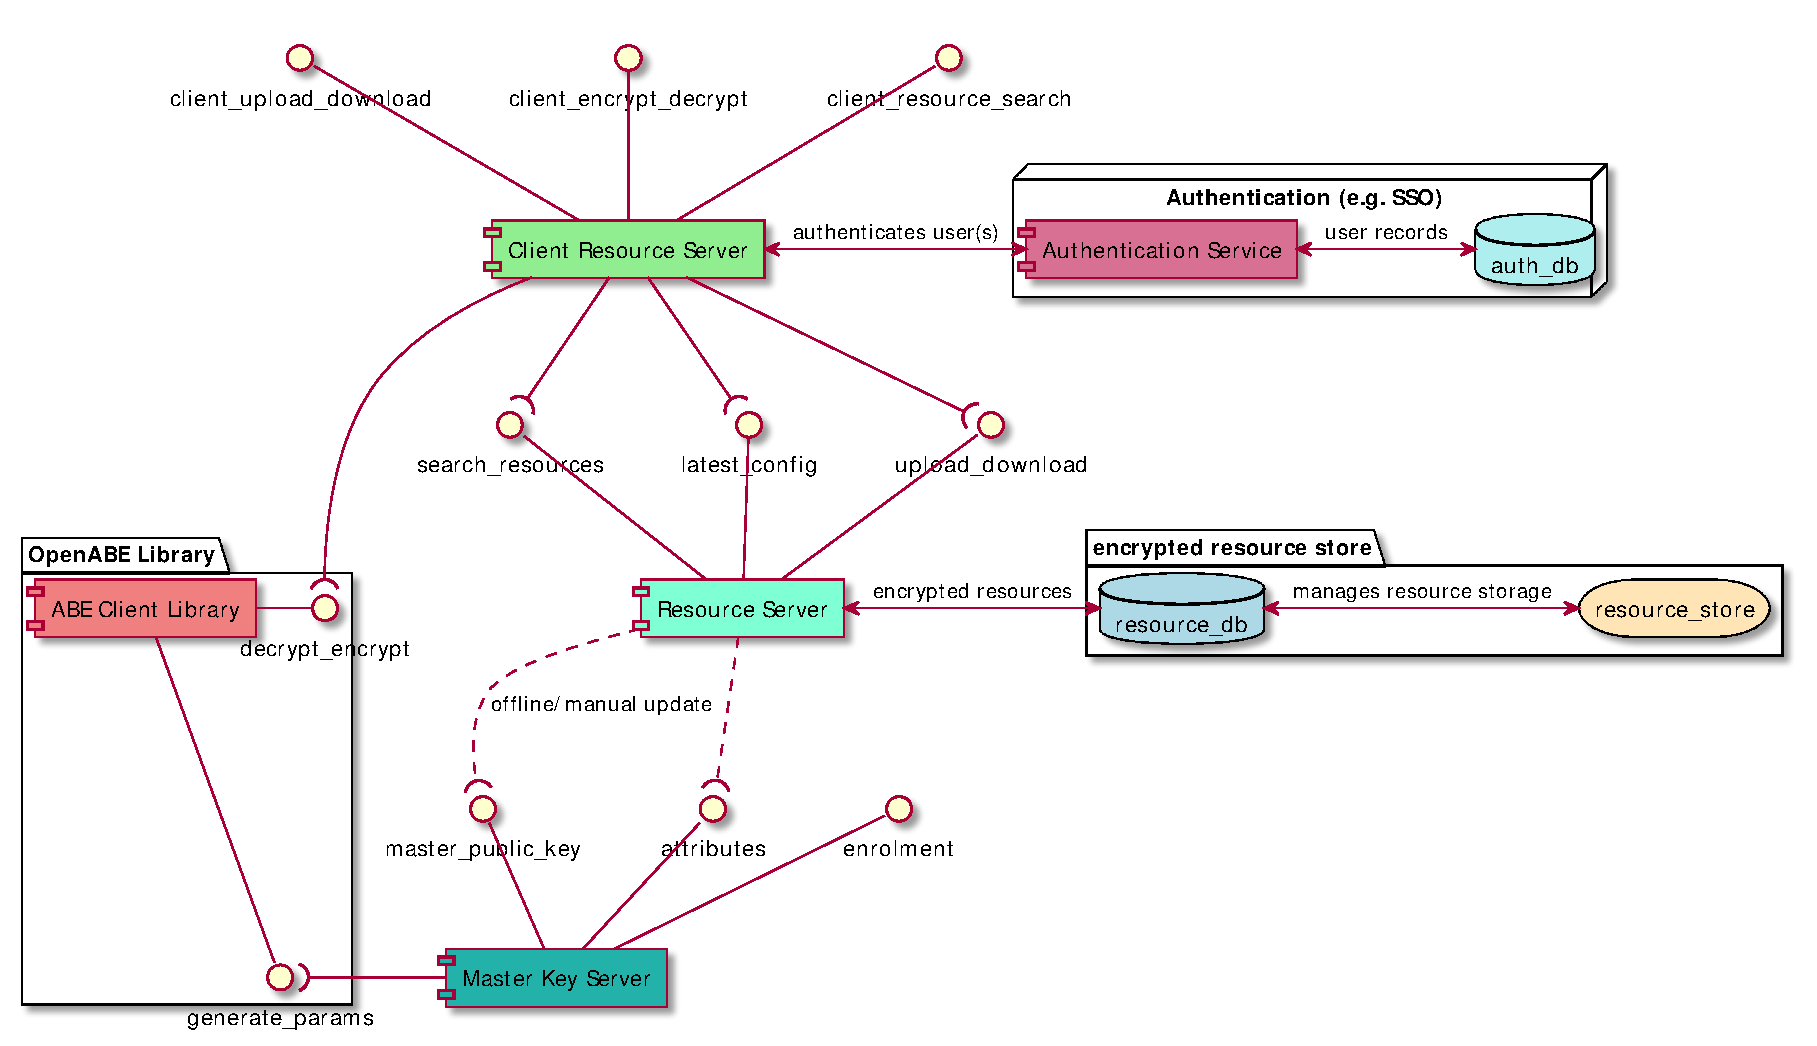
\includegraphics[width=\linewidth,keepaspectratio]{images/infrastructure/system_architecture_abbrv.pdf}

    \caption{
      \label{fig:sys_arch_abbrv}
      A condensed architecture diagram describing the system architecture of the \theResServer system. The \acrfull{mks} is shown in an offline state with access to a local copy of the \OpenABE library for provisioning the system \& generating user keys. The \acrfull{prs} is shown receiving offline updates from the \acrshort{mks}, managing a local database with resource metadata \& the associated resource storage and providing search, config and upload \& download interfaces for clients. The \acrfull{crs} is shown with local access to an \OpenABE library for encryption \& decryption and access to an abstract Authentication Service (such as the university's SSO system). The \acrshort{crs} also implements the search, config and upload \& download interfaces provided by the \acrshort{prs} and provides its own upload \& download, encrypt \& decrypt and resource search interfaces for the user.
    }

\end{figure}


\section{Policy Building}
\label{sec:design_pol_build}

The most complex aspect of using the \theResServer system for a user is the creation of policies for resources that the user wants to encrypt \& upload. For example, a user doesn't necessarily know all the attributes that have been signed into user keys (since they are extensible) and even if they have access to a list of attributes, they may not know which values are valid for a given attribute. Further complications arise from the fact that policies written in \thePolicyLang are then interpreted to \PyOpenABE as described in \cref{subsec:interpretation}.\\
Since we cannot expect a user to read the formal language definition for \thePolicyLang (\cref{sec:formal_lang}), as it is a technical definition, we need to provide a tool for a user to build policies with. This tool needs to inform the user of all currently assigned attributes and the possible values an attribute may accept, ensuring a comparable use of attributes across all policies. The tool needs to be user friendly and capable of enforcing correct types on the values the user inputs. Lastly, the tool should be generate a \thePolicyLang policy from the inputs and then generate the interpreted result of said \thePolicyLang policy, finally returning a \PyOpenABE-compatible policy.
\vskip 0.5em
Appendix \ref{appendix:policy_building} presents a screenshot of the resulting \acrshort{html}-based policy builder, as implemented for the \acrshort{crs}, and \cref{fig:policy_builder} specifically shows the result of building the policy required for Case Study \#1 (\cref{fig:case_study_policy_1}). The tool allows the user to build the policy line-by-line using dropdown fields that are pre-populated with the current attributes in use by the \theResServer system, which are collected from the \acrshort{prs}. The \acrshort{prs} in turn receives them via offline updates by \acrshort{dcs} Admins staff members from the \acrshort{mks}.\\
Per attribute selected by the user, a \acrshort{html} input field is created that enforces the type for the value the user must input via \acrshort{html}5 form validation \citep{Foundation2019}. The user can then `calculate' the resulting policy and a \PyOpenABE compiant policy is returned in textbox for the user to verify. If the policy is as expected, the user can continue with encrypting their desired file, again using the \acrshort{crs} (see \cref{fig:policy_builder}) with the \PyOpenABE library of bindings.


\section{Filename Searching}
\label{sec:design_file_search}

Users of the \theResServer system need to be able to identify resources they wish to download from the \acrfull{prs}. This may be trivial at first, since when there are only a few resources uploaded a user can easily browse a list to find the resources they need, however this quickly becomes infeasible as the \acrshort{prs} starts to store \textit{100s} of resources. Given the scale of the \acrfull{dcs}, this will become an issue quickly and so an alternative method of finding resources is required. Hence, we introduce a search utility for the \acrshort{prs}.
\vskip 0.5em
As described in \Cref{subsec:design_resources}, the \acrshort{prs} stores the metadata of uploaded resources in a local database to maintain a complete unawareness of the contents of any resources. An advantage to this design, is that the database can be efficiently queried for complex searches over all resources uploaded, requiring no storage operations by the \acrshort{prs}'s \acrshort{os}\@. Additionally, in future the metadata stored for each resource can easily be expanded to meet the evolving needs of the \acrshort{dcs}.

The \acrfull{crs} implements the search utilities offered by the \acrshort{prs}, offering resource searching directly to the user, with the added benefit of obscuring resources that the user would not be able to decrypt. This is possible as the \acrshort{crs} is aware of the user's assigned attributes and the \acrshort{prs} records the policy of every resource in its database at upload-time, allowing for quick checks of a user's attributes against a resource's policy.
\vskip 0.5em
The \theResServer system is designed to implement a simple filename search utility with the possibility to extend searching to include any of the other metadata stored for resources in the future.

The filename searching itself is to operate in one of two methods, either by directly matching a slice of a filename and returning a sorted list of the most likely matches (e.g. the query \textit{``report.pdf''} would match the filename \texttt{one\_example\_report.pdf} but not \texttt{one\_example\_report.docx}) or in a fuzzy finder method which would more generally score the similarities between a query and all available filenames, returning a sorted list of the most likely matches (e.g. the query \textit{``pdf apple report four''} would match highly with the filenames \texttt{report\_hci\_four\_final.pdf} \& \texttt{rep\_on\_four\_apples.docx}).


%==================================================================================================================================
\chapter{Implementation}
\label{ch:implementation}

%==================================================================================================================================
\chapter{Evaluation}
\label{ch:evaluation}
How good is your solution? How well did you solve the general problem, and what evidence do you have to support that?

%==================================================================================================================================
\chapter{Conclusion}
\label{ch:conclusion}
Summarise the whole project for a lazy reader who didn't read the rest (e.g. a prize-awarding committee).
\section{Guidance}
\begin{itemize}
    \item
        Summarise briefly and fairly.
    \item
        You should be addressing the general problem you introduced in the
        Introduction.
    \item
        Include summary of concrete results (``the new compiler ran 2x
        faster'')
    \item
        Indicate what future work could be done, but remember: \textbf{you
        won't get credit for things you haven't done}.
\end{itemize}

%==================================================================================================================================
%
%
%==================================================================================================================================
%  APPENDICES

\begin{appendices}

\chapter{Appendices}
\label{ch:appendices}

\section{Appendix A - Deployment Roles \& Users}
\label{appendix:roles_users}

\Cref{fig:appendix_roles_users} presents the identified user roles of the \acrfull{dcs} in red, to the left, and the identified users in blue, to the right. Also see (Electronic Appendix \ref{appendix:e_roles_users}).

\begin{figure}[htp]
    \centering
    \label{fig:appendix_roles_users}
    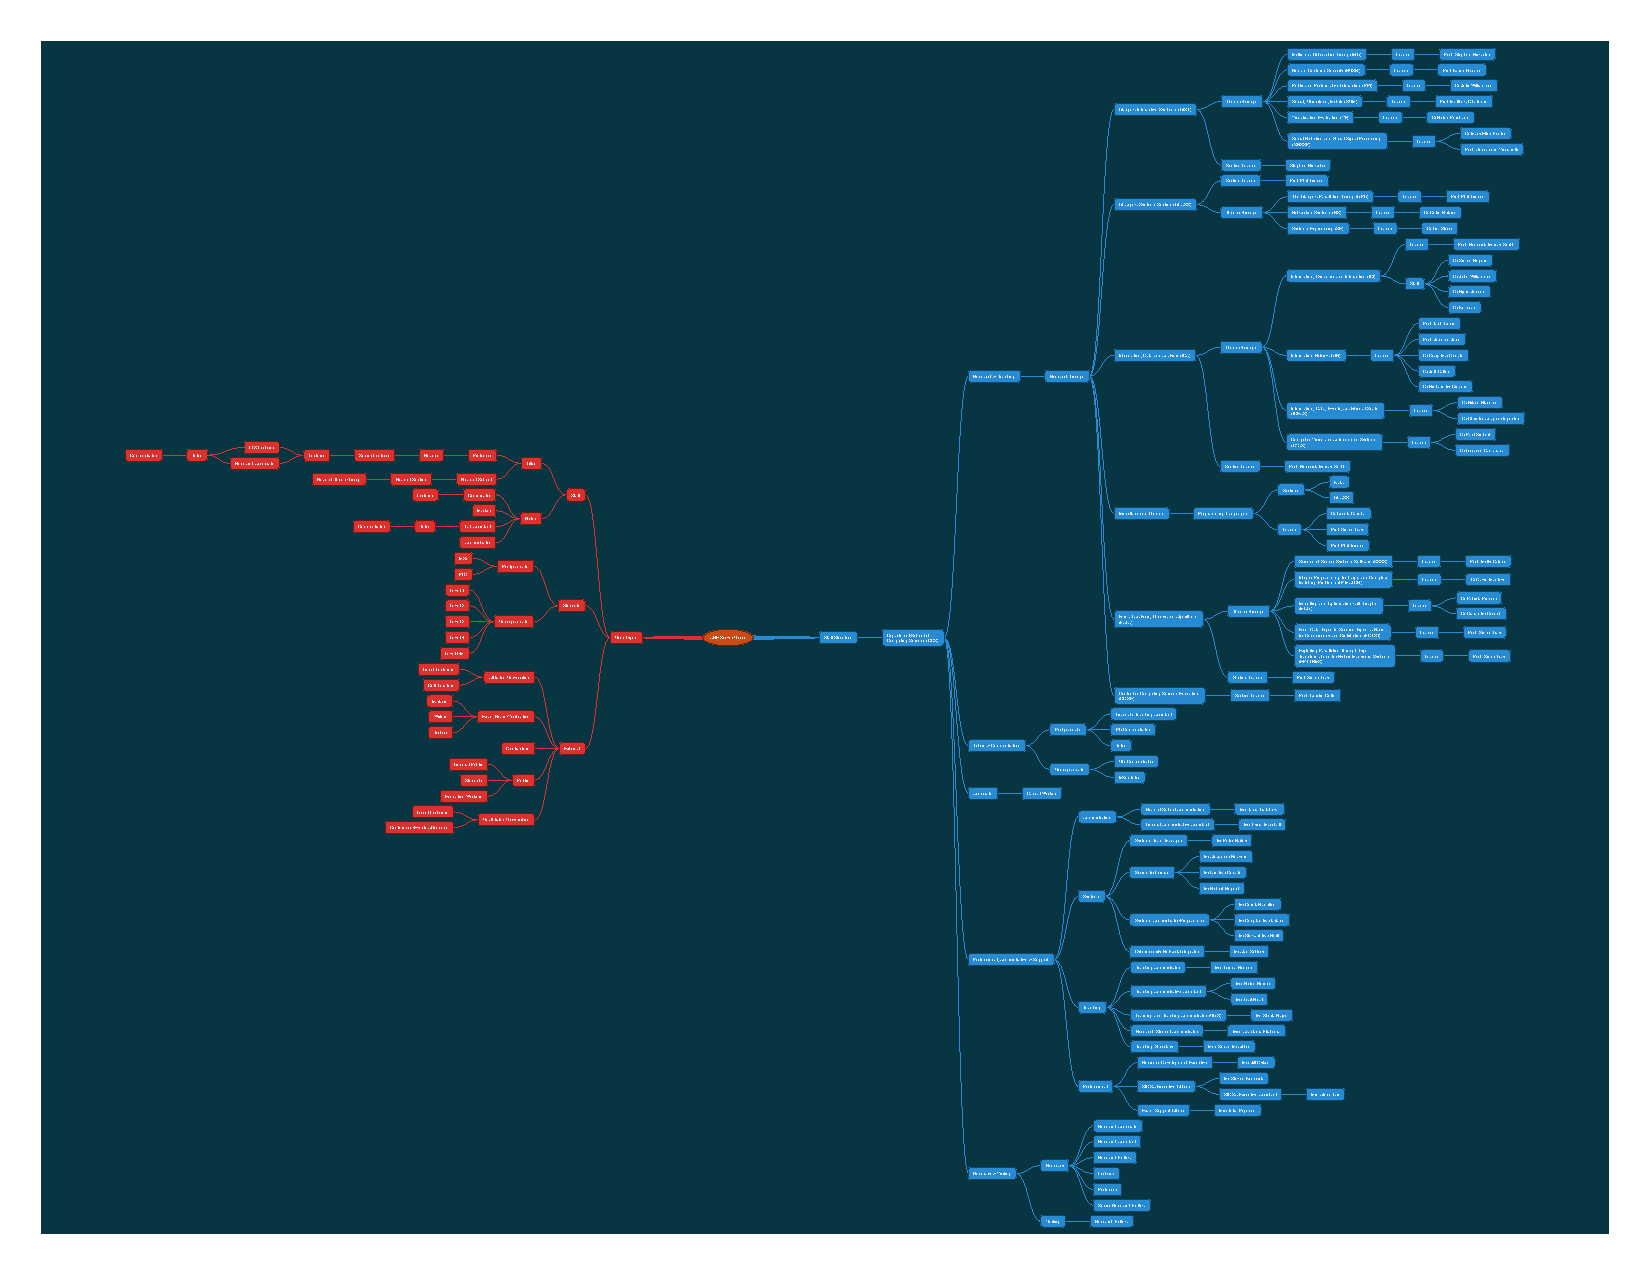
\includegraphics[width=\linewidth]{appendices/mind_maps/ABE_Users_slides_Oct26.pdf}
    \caption{Mind Map representing the different users \& roles identified for a \acrshort{dcs} deployment.}
\end{figure}

\section{Appendix B - Environment Attributes}
\label{appendix:environments}

\Cref{fig:appendix_environments} presents the identified environment attributes for the \acrfull{dcs}. Also see (Electronic Appendix \ref{appendix:e_environments}).

\begin{figure}[htp]
    \centering
    \label{fig:appendix_environments}
    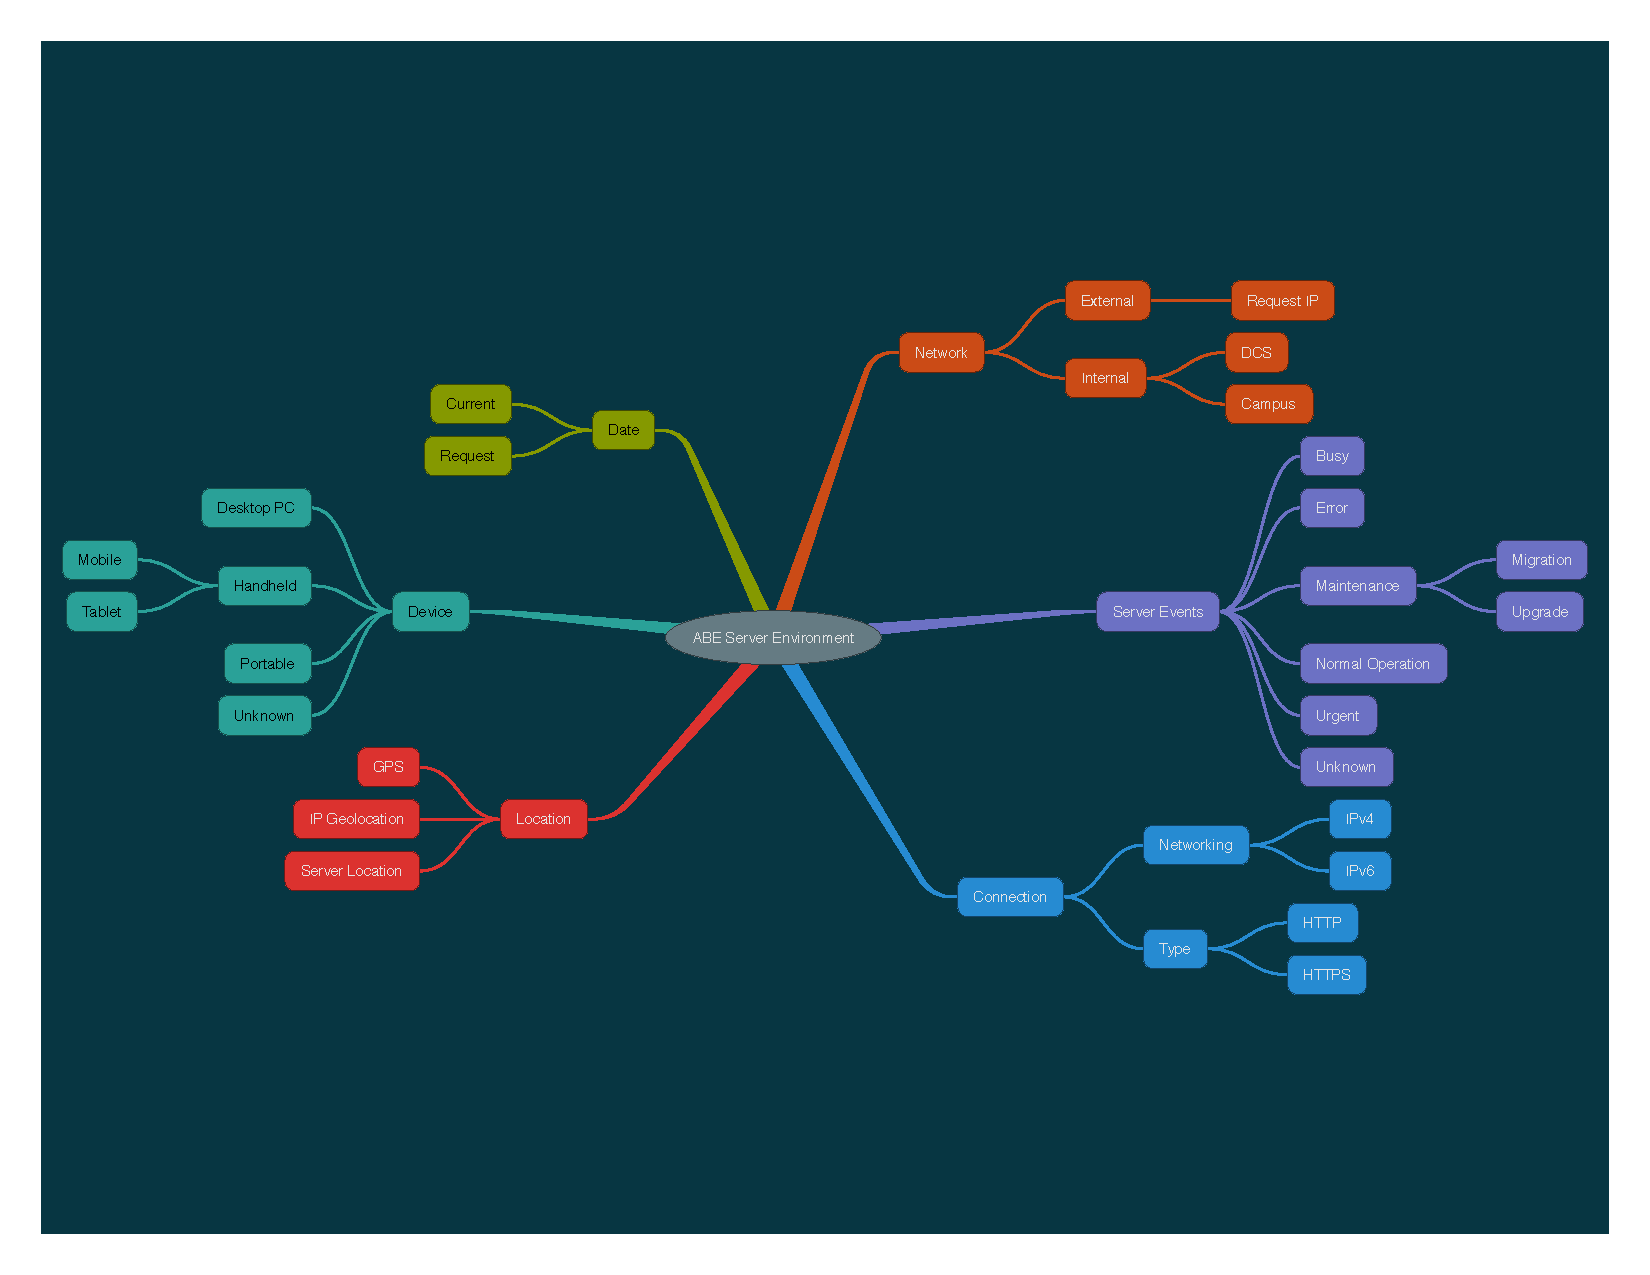
\includegraphics[width=\linewidth]{appendices/mind_maps/ABE_Environments_slides_Oct26.pdf}
    \caption{Mind Map representing the different environment attributes identified for a \acrshort{dcs} deployment.}
\end{figure}

\section{Appendix C - System Use Cases}
\label{appendix:use_cases}

\Cref{fig:appendix_use_cases} presents the identified use cases for the \acrfull{dcs}. Also see (Electronic Appendix \ref{appendix:e_use_cases}).

\begin{figure}[htp]
    \centering
    \label{fig:appendix_use_cases}
    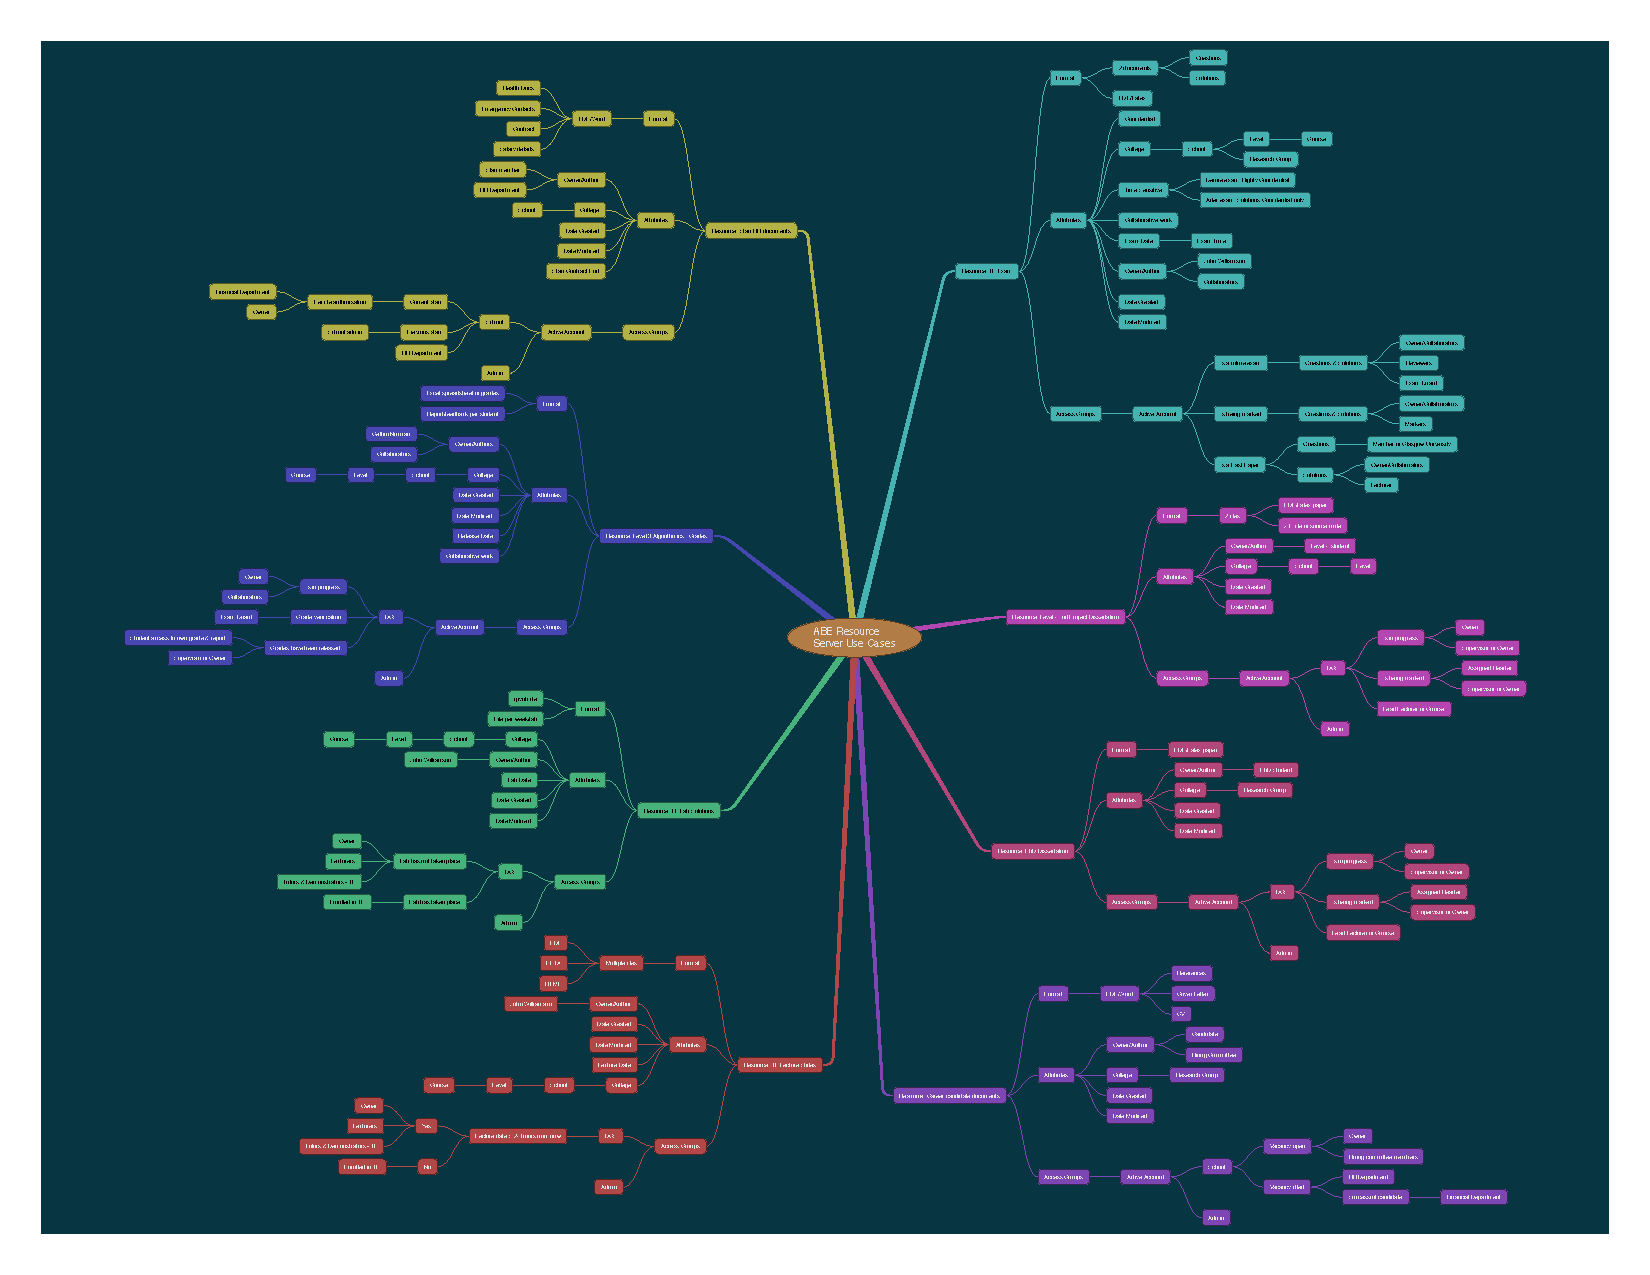
\includegraphics[width=\linewidth]{appendices/mind_maps/ABE_Use_Cases_slides_Oct26.pdf}
    \caption{Mind Map representing the different use cases identified for a \acrshort{dcs} deployment.}
\end{figure}

\section{Appendix D - Enrolment Diagram for Staff User}
\label{appendix:enrolment_diagram}

\Cref{fig:appendix_sta_deployment} represents a deployment diagram for the \theResServer system, with staff member enrolling into the system. This diagram is an alternative to the student enrolment diagram in \Cref{fig:deployment_diagram}.

The staff member can be seen requesting a user key \#1 (and providing their staff username) from the \acrshort{dcs} Teaching Assistant, whom verifies the staff members's identity and then retrieves their details \#2 from the HR/Payroll system. The Teaching Assistant then processes the returned attributes \#5 for the Master Key Server, and then requests a new key \#6 by providing the student's attributes. The Master Key Server can be seen processing \#7 and then returning the newly generated key \#8 to the Teaching Assistant, whom finally provides the key to the staff member.

\begin{figure}[htp]
    \centering
    \label{fig:appendix_sta_deployment}
    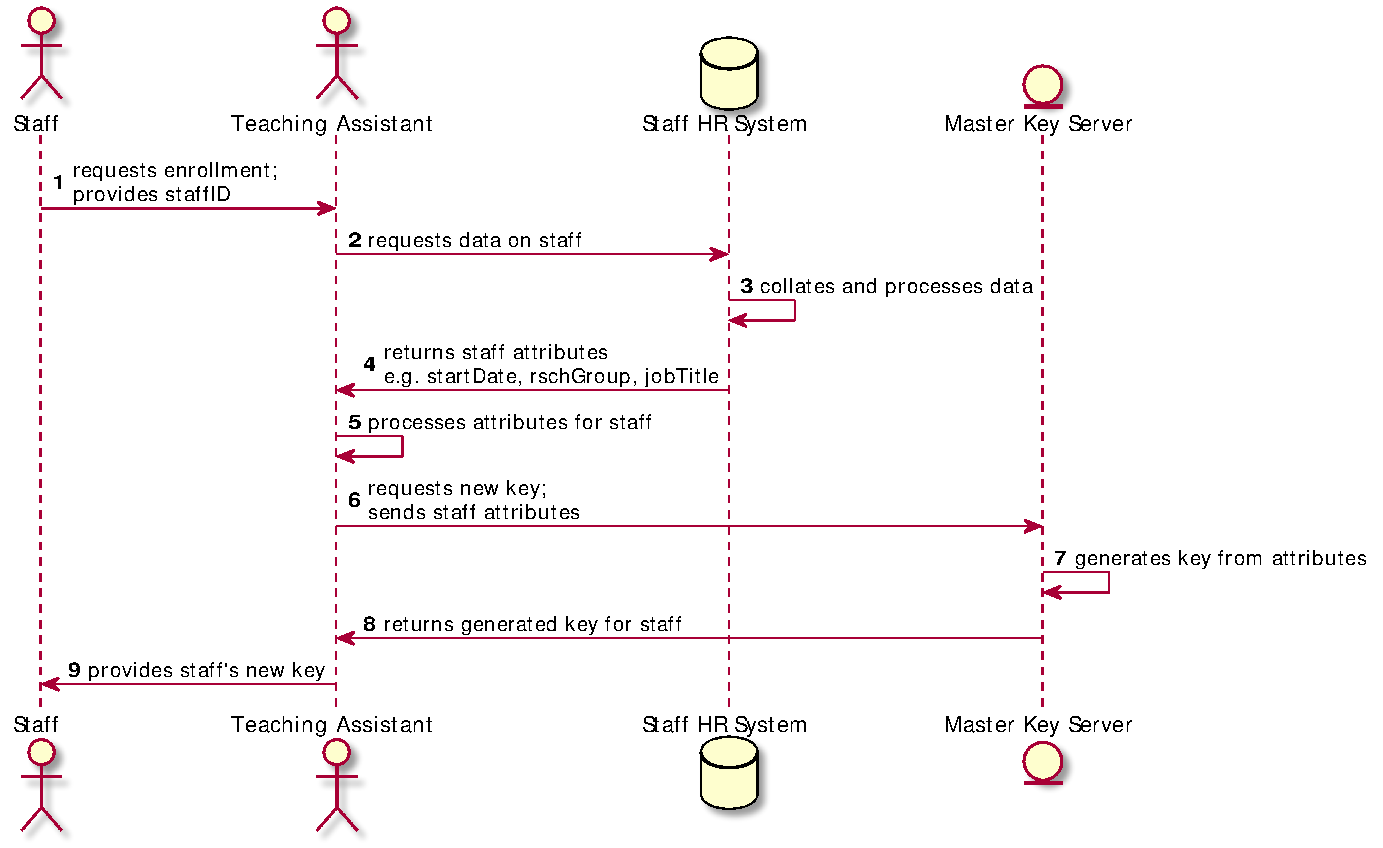
\includegraphics[width=\linewidth,keepaspectratio]{appendices/diagrams/flow_of_info/enrollment_sta_sequence.pdf}

    \caption{A sequence diagram demonstrating the enrolment process for a staff member.}

\end{figure}

\section{Appendix E - System Architecture Diagram}
\label{appendix:architecture_diagram}

\Cref{fig:appendix_sys_arch_full} represents a system architecture diagram for the \theResServer system. This diagram is an alternative to the condensed system architecture diagram in \Cref{fig:sys_arch_abbrv}.

The \acrfull{mks} is shown in an offline state with access to a local copy of the \OpenABE library for provisioning the system \& generating user keys. The \acrfull{prs} is shown receiving offline updates from the \acrshort{mks}, managing a local database with resource metadata \& the associated resource storage and providing search, config and upload \& download interfaces for clients. The \acrfull{crs} is shown with local access to an \OpenABE library for encryption \& decryption and access to an abstract Authentication Service (such as the university's SSO system). The \acrshort{crs} also implements the search, config and upload \& download interfaces provided by the \acrshort{prs} and provides its own upload \& download, encrypt \& decrypt and resource search interfaces for the user.

\begin{figure}[htp]
    \centering
    \label{fig:appendix_sys_arch_full}
    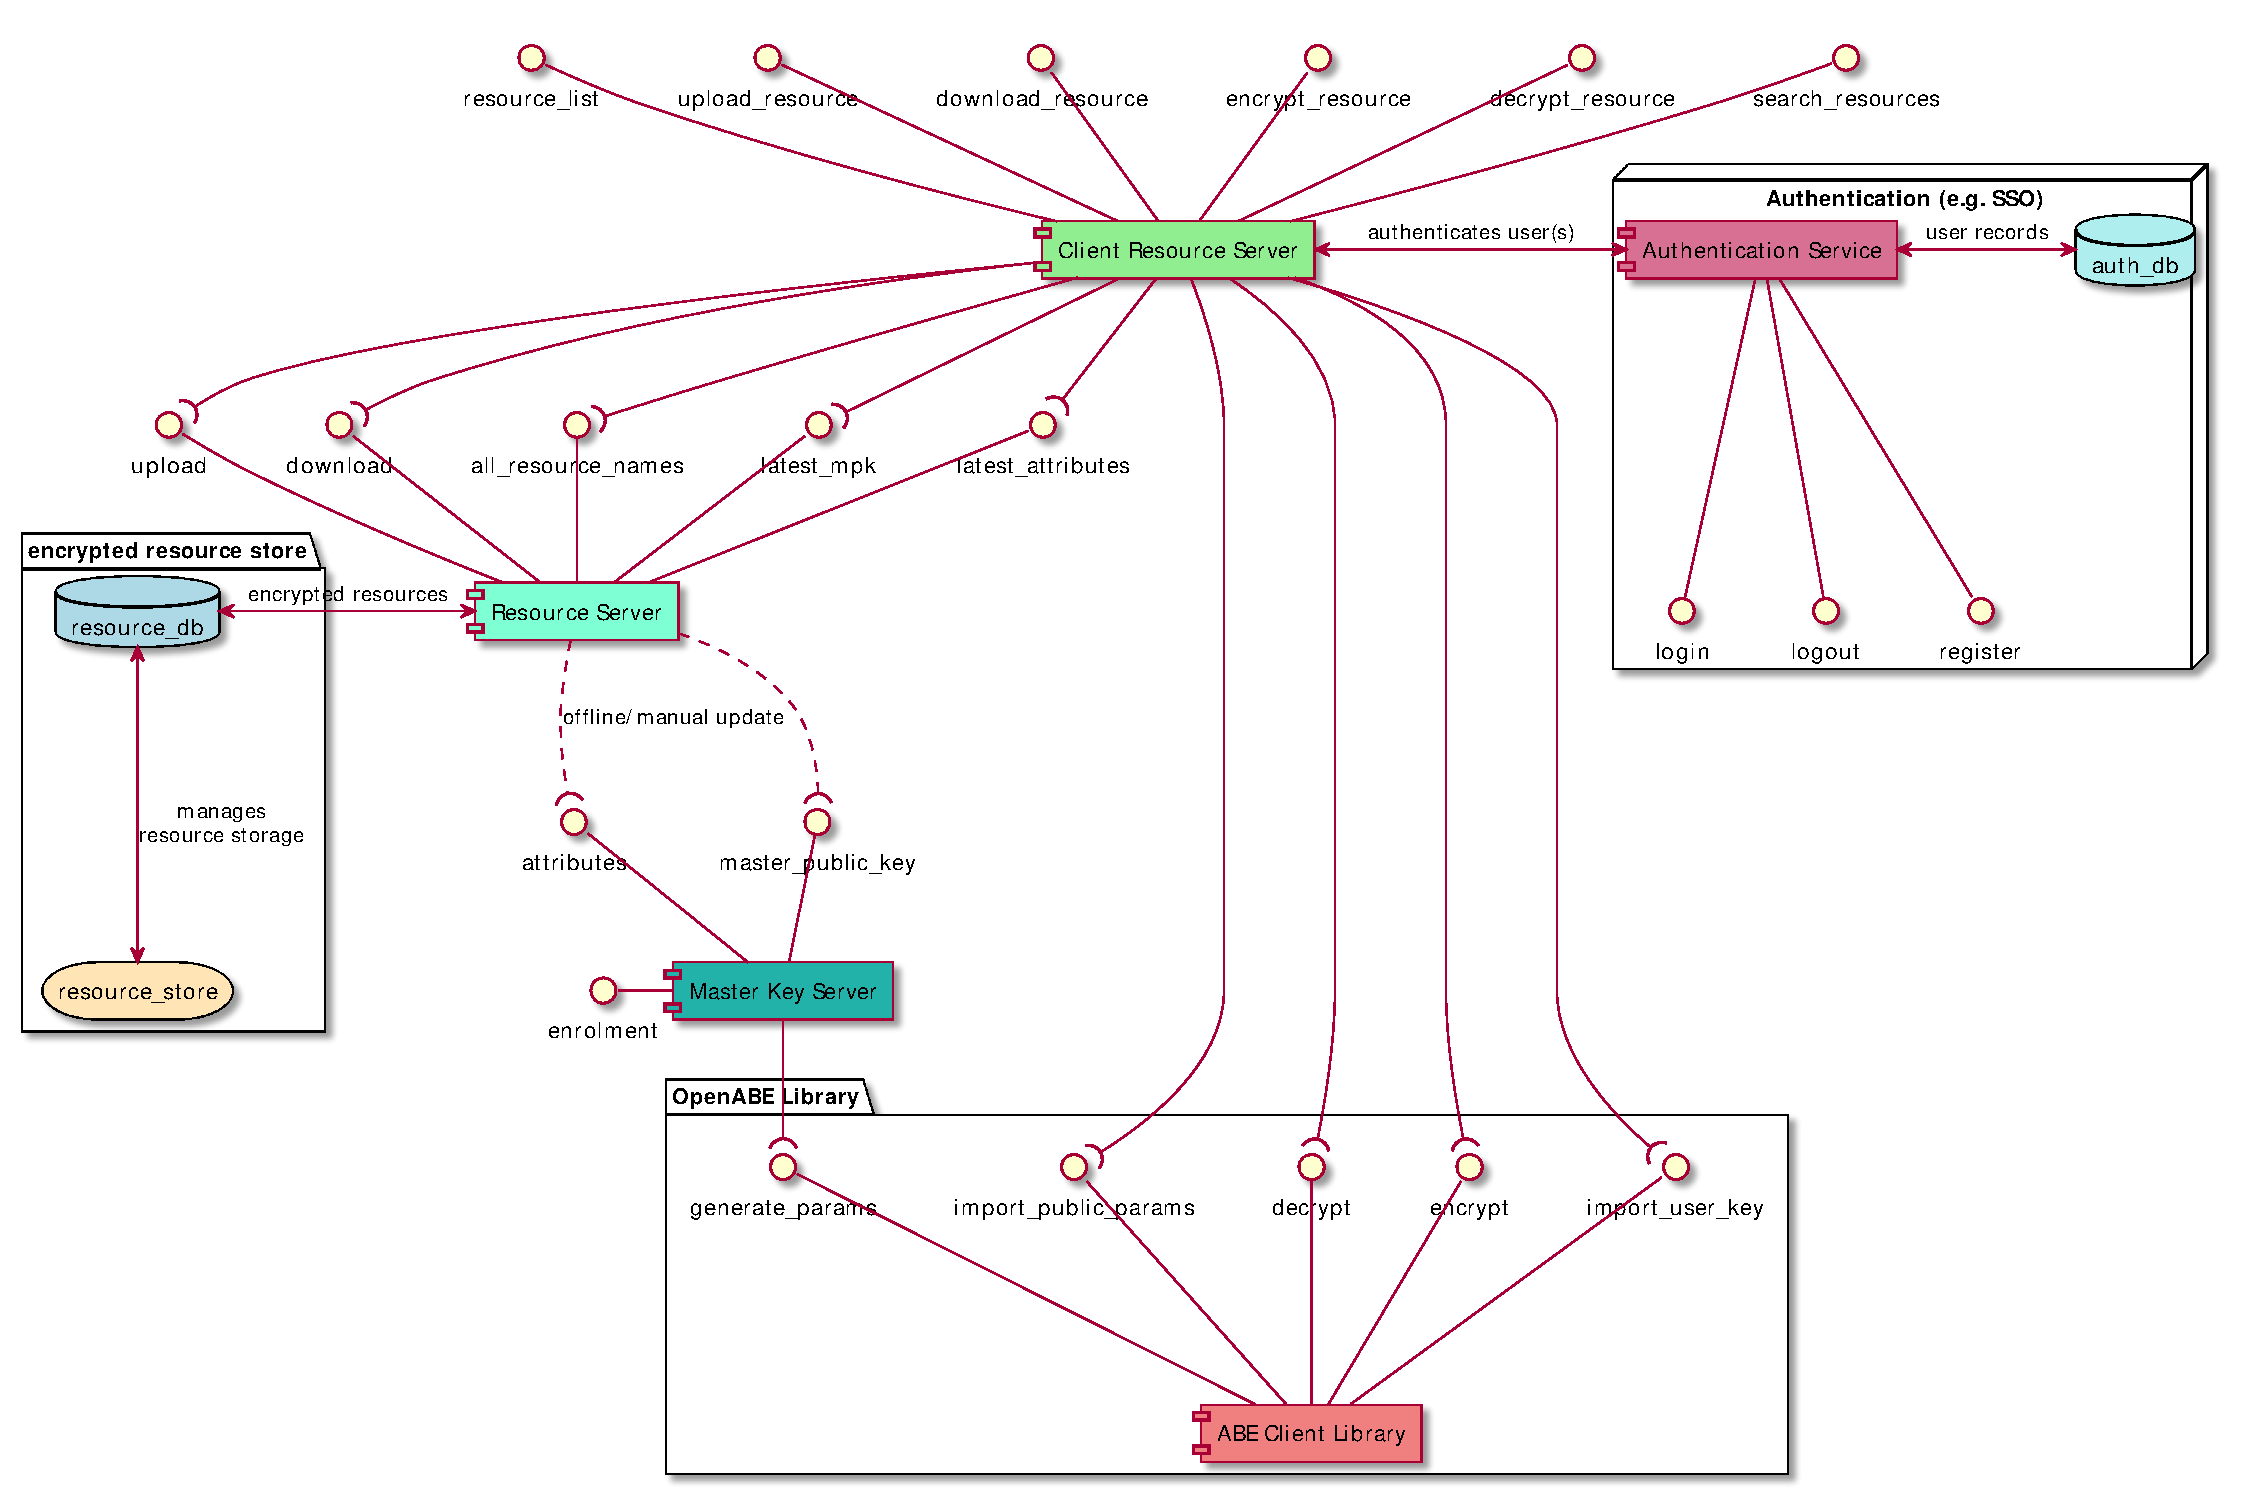
\includegraphics[width=\linewidth,keepaspectratio]{appendices/diagrams/infrastructure/system_architecture.pdf}

    \caption{
      A full architecture diagram describing the system architecture of the \theResServer system.
    }

\end{figure}

\section{Appendix F - Implementing Case Study \#0 with \thePolicyLang}
\label{appendix:case_study_0_policy}

For this study the following details have been assumed:
\begin{itemize}
  \item
    the solutions were encrypted and then uploaded by the Admin staff member
  \item
    the staff member is Teresa Bonner with username `tbonner'
\end{itemize}
\vskip 0.5em
With the details extracted, we can determine the attributes for the policy, where we define \textbf{\textit{Subject} s} and \textbf{\textit{Environment} e} as:
\begin{itemize}
  \item[]
    \textbf{s} $\Rightarrow$ role, accountActiveUntil, username
  \item[]
    \textbf{e} $\Rightarrow$ currentDate
\end{itemize}

Applying the identified attributes for Case Study \#0 (\Cref{subsec:analysis_case_studies_0}) provides the policy in \cref{fig:case_study_policy_0} which would have been embedded in the encrypted lecture slides by the staff member before upload. The encrypted past paper can then remain stored on the server but only accessible to staff members and students.

\begin{figure}[ht]
  \centering
\begin{align*}
  \text{Policy(\textbf{s},\textbf{e})}
  &
    \leftarrow
    \text{username(\textbf{s})} \equiv \text{`tbonner'}
  \\
  &
    \phantom{::}\vee
    \text{role(\textbf{s})} \equiv \text{`Staff'} \mid \text{`Student'}
  \\
  &
    \phantom{::}\wedge
    \text{accountActiveUntil(\textbf{s})} \geq \text{currentDate(\textbf{e})}
\end{align*}
  \caption{
    \label{fig:case_study_policy_0}
    Case Study \#0 policy dictating access to a past exam paper.
    Successful decryption would be possible for the author of the slides (with username `tbonner') \textbf{or} any member of staff \textbf{or} any student. In all cases an active account is also required.
  }
\end{figure}


\section{Appendix G - Implementing Case Study \#2 with \thePolicyLang}
\label{appendix:case_study_2_policy}

For the sake of the scenario, the 1P Programming course was selected with Course Code 1001 as it offers the added complexity of tutors \& demonstrators, but it should be remembered that any course with labs could have been chosen.
\vskip 0.5em
For this study the following details have been assumed:
\begin{itemize}
  \item
    the lab solutions have been uploaded in advance of the actual lab date
  \item
    the lab date is scheduled for 04/12/19
  \item
    the solutions were encrypted and then uploaded by the Lecturer
  \item
    the Lecturer for 1001 is John Williamson with username `jwilliamson'
  \item
    Course 1001 is a Level 1 course
  \item
    Course 1001 has a sister course, 1017
  \item
    the 1P course labs are assisted by tutors \& demonstrators from Level 4+
\end{itemize}

\begin{figure}[ht]
  \centering
\begin{align*}
  \text{Policy($sub$, $env$, $res$)}
  &
    \leftarrow
    \text{username($sub$)} \equiv \text{`jwilliamson'}
  \\
  &
    \phantom{::}\vee
    \text{( role($sub$)} \equiv \text{`Staff'}
  \\
  &
    \phantom{::::::::}\wedge
    \text{jobField($sub$)} \equiv \text{`Research \& Teaching' )}
  \\
  &
    \phantom{::}\vee
    \text{( role($sub$)} \equiv \text{`Student'}
  \\
  &
    \phantom{::::::::}\wedge
    \text{studentLevel($sub$)} \equiv \text{1}
  \\
  &
    \phantom{::::::::}\wedge
    \text{enrolledCourses($sub$)} \equiv \text{[1001, 1017]}
  \\
  &
    \phantom{::::::::}\wedge
    \text{currentDate($env$)} \geq \text{7 December 2019 )}
  \\
  &
    \phantom{::}\vee
    \text{( role($sub$)} \equiv \text{`Student'}
  \\
  &
    \phantom{::::::::}\wedge
    \text{studentLevel($sub$)} \geq \text{4}
  \\
  &
    \phantom{::::::::}\wedge
    \text{studentRole($sub$)} \equiv \text{`Demonstrator UG'} \mid \text{`Demonstrator PG'} \mid \text{`Tutor'}
  \\
  &
    \phantom{::::::::}\wedge
    \text{demonstratorCourses($sub$)} \equiv \text{[1001, 1017]}
  \\
  &
    \phantom{::::::::}\wedge
    \text{startDate($env$)} \leq \text{currentDate($env$)}
  \\
  &
    \phantom{::::::::}\wedge
    \text{endDate($env$)} \geq \text{currentDate($env$) )}
  \\
  &
    \phantom{::}\wedge
    \text{accountActiveUntil($sub$)} \geq \text{currentDate($env$)}
\end{align*}
  \caption{
    \label{fig:case_study_policy_2}
    Case Study \#2 policy dictating access to a set of course `1001' lab solutions.
  }
\end{figure}
Applying the identified attributes for Case Study \#2 provides the policy in \Cref{fig:case_study_policy_2} which would have been embedded in the encrypted lab solution by the Lecturer before upload. The encrypted lab solution can then remain stored on the server but will only accessible to the author of the solutions (with username `jwilliamson') \textbf{or} a member of staff in the `Research \& Teaching' field \textbf{or} a Level 2 student enrolled in the `1001' \& `1017' courses if it is 3 days after the lab date of 04/12/19 \textbf{or} a Level 4+ student employed as a demonstrator or tutor that has been assigned to the `1001' \& `1017' course and it is within their dates of employment. In all cases an active account is also required.


\section{Appendix H - Implementing Case Study \#3 with \thePolicyLang}
\label{appendix:case_study_3_policy}

For the sake of the scenario, the Programming Languages course was selected with Course Code 4016 to show the creation of a policy.
\vskip 0.5em
For this study the following details have been assumed:
\begin{itemize}
  \item
    the exam script is a work in progress resource
  \item
    the exam script has been uploaded in advance of the exam date
  \item
    the solutions were encrypted and then uploaded by the Lecturer
  \item
    the Lecturer's Research Group is FATA
  \item
    the Lecturer's Research Theme\slash Topic is Programming Languages
  \item
    the exam date is 12/05/20
  \item
    the marking deadline is 10/06/20
  \item
    the Lecturer for 4016 is Ornela Dardha with username `odardha'
  \item
    collaborators include Simon Gay (`sgay'), John O'Donnell (`jodonnell')
\end{itemize}
\vskip 0.5em
Applying the identified attributes for Case Study \#3 provides the policy in \Cref{fig:case_study_policy_3} which would have been embedded in the encrypted exam script by the Lecturer before upload. The encrypted exam script can then remain stored on the server but would only be the Lecturer themselves, as well as the specified collaborators.

Further access would be granted to staff members in the Professional, Administrative \& Support field that specifically have the Administration role, as well as Research \& Teaching staff members that belong to the FATA research group and the Programming Languages research theme. Lastly, access would be granted to markers that have been assigned to the 4016 course and will be actively marking during the marking period (12/05/20\textemdash10/06/20).

\begin{figure}[ht]
  \centering
\begin{align*}
  \text{Policy($sub$, $env$, $res$)}
  &
    \leftarrow
    \text{username($sub$)} \equiv \text{`odardha'} \mid \text{`sgay'} \mid \text{`jodonnell'}
  \\
  &
    \phantom{::}\vee
    \text{( role($sub$)} \equiv \text{`Staff'}
  \\
  &
    \phantom{::::::::}\wedge
    \text{jobField($sub$)} \equiv \text{`Professional, Administrative \& Support'}
  \\
  &
    \phantom{::::::::}\wedge
    \text{jobRole($sub$)} \equiv \text{`Administration' )}
  \\
  &
    \phantom{::}\vee
    \text{( role($sub$)} \equiv \text{`Staff'}
  \\
  &
    \phantom{::::::::}\wedge
    \text{jobField($sub$)} \equiv \text{`Research \& Teaching'}
  \\
  &
    \phantom{::::::::}\wedge
    \text{researchGroup($sub$)} \equiv \text{`FATA'}
  \\
  &
    \phantom{::::::::}\wedge
    \text{researchTheme($sub$)} \equiv \text{`Programming Languages' )}
  \\
  &
    \phantom{::}\vee
    \text{( role($sub$)} \equiv \text{`Staff'}
  \\
  &
    \phantom{::::::::}\wedge
    \text{staffRole($sub$)} \equiv \text{`Marker'}
  \\
  &
    \phantom{::::::::}\wedge
    \text{markerFrom($sub$)} \geq \text{12 May 2020}
  \\
  &
    \phantom{::::::::}\wedge
    \text{markerTo($sub$)} \leq \text{10 June 2020}
  \\
  &
    \phantom{::::::::}\wedge
    \text{markerCourses($sub$)} \equiv \text{4016}
  \\
  &
    \phantom{::}\wedge
    \text{accountActiveUntil($sub$)} \geq \text{currentDate($env$)}
\end{align*}
  \caption{
    \label{fig:case_study_policy_3}
    Case Study \#3 policy dictating access to a work-in-progress exam script for course `4016'.
    Successful decryption would be possible for the author of the solutions (with username `odardha') as well as the named collaborators (with usernames `sgay' \& `jodonnell') \textbf{or} for a member of staff in the `Professional, Administrative \& Support' field with the `Administration' role \textbf{or} for a member of staff in the `Research \& Teaching' field that is also in the `FATA' research group and the `Programming Languages' research theme \textbf{or} for a member of staff with the `Marker' role that is assigned to marking duties within the marking period and has been assigned to the `4016' course. In all cases an active account is also required.
  }
\end{figure}


\section{Appendix I - Implementing Case Study \#4 with \thePolicyLang}
\label{appendix:case_study_4_policy}

In this case, the student has encrypted and uploaded their dissertation to the \theResServer system with access to be granted for their supervisor, the assigned reader and additionally, the Project Coordinator.
\vskip 0.5em
For this study the following details have been assumed:
\begin{itemize}
  \item
    the student has the ID and username `2123456z'
  \item
    their supervisor is Quintin Cutts with username `qcutts'
  \item
    their assigned reader is Paul Siebert with username `psiebert'
  \item
    the Project Coordinator is John Williamson with username `jwilliamson'
\end{itemize}
\vskip 0.5em
Applying the identified attributes for Case Study \#4 provides the policy in \Cref{fig:case_study_policy_4} which would have been embedded in the encrypted dissertation by the student before upload. The encrypted dissertation can then remain stored on the server but only accessible to the student and required staff members.

\begin{figure}[ht]
  \centering
\begin{align*}
  \text{Policy($sub$, $env$, $res$)}
  &
    \leftarrow
    \text{( role($sub$)} \equiv \text{`Student'}
  \\
  &
    \phantom{::::::}\wedge
    \text{username($sub$)} \equiv \text{`2123456z' )}
  \\
  &
    \phantom{::}\vee
    \text{( role($sub$)} \equiv \text{`Staff'}
  \\
  &
    \phantom{::::::}\wedge
    \text{username($sub$)} \equiv \text{`qcutts'} \mid \text{`psiebert'} \mid \text{`jwilliamson' )}
  \\
  &
    \phantom{::}\wedge
    \text{accountActiveUntil($sub$)} \geq \text{currentDate($env$)}
\end{align*}
  \caption{
    \label{fig:case_study_policy_4}
    Case Study \#4 policy dictating access to a completed dissertation.
    Successful decryption would be possible for the author of the dissertation (with username `2123456z') \textbf{or} for the three identified staff members (with usernames `qcutts', `psiebert', `jwilliamson'). In all cases an active account is also required.
  }
\end{figure}


\section{Appendix J - Physical Assets for Master Key Server}
\label{appendix:mks_assets}

\begin{table}[htp]
  \rowcolors{2}{}{gray!3}
  \begin{tabularx}{\linewidth}{lX}
    \textbf{Asset}          & \textbf{Description} \\
    Router or Switch        &	Router (AP) or Switch host is connected to (if host is not offline). \\
    Network connection      &	Physical connection to network (if host not offline). \\
    Storage                 &	Storage for host, high risk, contains keys, config, server files etc. \\
    Monitor                 &	General output for host, low risk. \\
    Keyboard                &	General input for host, low risk. \\
    Mouse                   &	General input for host, low risk. \\
    Computer                &	The actual host machine of the server. \\
    Room key                &	Simply the key that grants access to the physical room the server is located in. \\
    Building                &	The physical building the host machine is located in. \\
    Room                    &	The physical room the host machine is located in. \\
    External Storage/Media  &	Any external storage/media attached to the host machine during operation. \\
  \end{tabularx}
  \caption{Physical assets for the \acrfull{mks}}
  \label{tab:physical_assets_mk}
\end{table}

\section{Appendix K - Assets for Public Resource Server}
\label{appendix:prs_assets}

\begin{table}[htp]
  \rowcolors{2}{}{gray!3}
  \begin{tabularx}{\linewidth}{lX}
    \textbf{Asset}            & \textbf{Description} \\
    Master Public Key file    &	Not dangerous, value is distributed as part of normal operation. \\
    Global Attributes file    &	As above, is distributed as part of normal operation but potentially reveals information on the system. \\
    Server Secret (sessions)  &	Secret used to set up sessions with users, and generate CSRF tokens. Potentially dangerous. \\
    Local web server files    &	Contains other config files, but also the key files. Needs protection. \\
    jinja2 plugin             &	Plugin to generate templates. Lowish risk, but an external party provides software. \\
    flask plugin              &	Tool to create and run a web server, potentially damaging. Produced and updated by an external party. \\
    PyMongo plugin            &	Plugin used by flask server to communicate with the Mongo DB. \\
    Python3 lib               &	The Python3 library. Similar to above, lower vulnerability as very openly and globally reviewed. \\
    MongoDB Database          & Database of resource meta data. \\
    MongoDB system            & System running MongoDB databases. Produced and updated by an external party. \\
    C lib                     &	The C library. Similar to Python, low vulnerability as extremely openly and globally reviewed. Slow to update as well. \\
    Resource files            & Encrypted ciphertexts representing the resources stored on the server. \\
    Firewall                  &	Firewall of the host. Should block incoming requests. May not even be necessary as Key Server should be offline when deployed. \\
    UNIX OS                   &	The UNIX OS the host is running on. External party software so potential risk.
  \end{tabularx}
  \caption{Virtual assets for the \acrfull{prs}}
  \label{tab:virtual_assets_pr}
\end{table}

\begin{table}[htp]
  \rowcolors{2}{}{gray!3}
  \begin{tabularx}{\linewidth}{lX}
    \textbf{Asset}          & \textbf{Description} \\
    Router or Switch        &	Router (AP) or Switch host is connected to. \\
    Network connection      &	Physical connection to network. \\
    Storage                 &	Storage for host, high risk, contains resources, config, server files etc. \\
    Computer                &	The actual host machine of the server. \\
    Building                &	The physical building the host machine is located in. \\
    Room                    &	The physical room the host machine is located in. \\
    External Storage/Media  &	Any external storage/media attached to the host machine during operation. \\
  \end{tabularx}
  \caption{Physical assets for the \acrfull{prs}}
  \label{tab:physical_assets_pr}
\end{table}

\section{Appendix L - Assets for Client Resource Server}
\label{appendix:crs_assets}

\begin{table}[htp]
  \rowcolors{2}{}{gray!3}
  \begin{tabularx}{\linewidth}{lX}
    \textbf{Asset}            & \textbf{Description} \\
    User Key                  & High risk. The end user's private key, used to decrypt all resources. \\
    Master Public Key file    &	Not dangerous, value is distributed as part of normal operation. \\
    Global Attributes file    &	As above, is distributed as part of normal operation but potentially reveals information on the system. \\
    Server Secret (sessions)  &	Secret used to set up sessions with users, and generate CSRF tokens. Potentially dangerous. \\
    Local web server files    &	Contains other config files, but also the key files. Needs protection. \\
    jinja2 plugin             &	Plugin to generate templates. Lowish risk, but an external party provides software. \\
    flask plugin              &	Tool to create and run a web server, potentially damaging. Produced and updated by an external party. \\
    PyMongo plugin            &	Plugin used by flask server to communicate with the Mongo DB. \\
    PyOpenABE bindings        &	Python bindings for decryption. High risk. Also maintained by external party. \\
    cython lib/plugin         &	Python tool to compile python down to C. Interprets all bindings. So as above. \\
    Python3 lib               &	The Python3 library. Similar to above, lower vulnerability as very openly and globally reviewed. \\
    OpenABE C lib             &	OpenABE library for all user key generation. High risk. Maintained by external party. \\
    MongoDB Database          & Database of resource meta data. \\
    MongoDB system            & System running MongoDB databases. Produced and updated by an external party. \\
    C lib                     &	The C library. Similar to Python, low vulnerability as extremely openly and globally reviewed. Slow to update as well. \\
    Resource files            & Decrypted resources downloaded from server. \\
    Firewall                  &	Firewall of the host. Up to user. \\
    UNIX OS                   &	The UNIX OS the host is running on. External party software so potential risk.
  \end{tabularx}
  \caption{Virtual assets for the \acrfull{crs}}
  \label{tab:virtual_assets_cr}
\end{table}

\begin{table}[htp]
  \rowcolors{2}{}{gray!3}
  \begin{tabularx}{\linewidth}{lX}
    \textbf{Asset}          & \textbf{Description} \\
    Router or Switch        &	Router (AP) or Switch host is connected to (if host is not offline). \\
    Network connection      &	Physical connection to network (if host not offline). \\
    Storage                 &	Storage for host, high risk, contains keys, config, server files etc. \\
    Monitor                 &	General output for host, low risk. \\
    Keyboard                &	General input for host, low risk. \\
    Mouse                   &	General input for host, low risk. \\
    Computer                &	The actual host machine of the server. \\
    External Storage/Media  &	Any external storage/media attached to the host machine during operation. \\
  \end{tabularx}
  \caption{Physical assets for the \acrfull{crs}}
  \label{tab:physical_assets_cr}
\end{table}

\section{Electronic Appendices}
\label{appendix:electronic_appendices}

\subsection{Appendix E1 - Deployment Roles \& Users}
\label{appendix:e_roles_users}

We make note of the Deployment Roles \& Users mind map document. Although contained in Appendix \ref{appendix:roles_users}, it is too large to be viewed fully within the dissertation, therefore it is included in the submitted code file under: \texttt{l4-project-research/Mind\_Maps/ABE\_Users.slides\_Oct26.pdf}.

\subsection{Appendix E2 - Environment Attributes}
\label{appendix:e_environments}

We make note of the Environment Attributes mind map document. Although contained in Appendix \ref{appendix:environments}, it is too large to be viewed fully within the dissertation, therefore it is included in the submitted code file under: \texttt{l4-project-research/Mind\_Maps/ABE\_Environments.slides\_Oct26.pdf}.

\subsection{Appendix E3 - System Use Cases}
\label{appendix:e_use_cases}

We make note of the system Use Cases mind map document. Although contained in Appendix \ref{appendix:use_cases}, it is too large to be viewed fully within the dissertation, therefore it is included in the submitted code file under: \texttt{l4-project-research/Mind\_Maps/ABE\_Use\_Cases.slides\_Oct26.pdf}.

\subsection{Appendix E4 - Risk Assessment}
\label{appendix:e_risk_assessment}

We make note of the Risk Assessment Excel document. Too large to submit within the dissertation, it is included in the submitted code file under: \texttt{l4-project-research/reports/RiskAssessment.xlsx}.

\end{appendices}


%==================================================================================================================================
%   BIBLIOGRAPHY

% The bibliography style is abbrvnat
% The bibliography always appears last, after the appendices.

\bibliographystyle{abbrvnat}

\bibliography{l4proj}

\newpage

\printnoidxglossaries

\end{document}
